\documentclass[12pt]{report}

% input characters
\usepackage[utf8]{inputenc}
\usepackage[T1]{fontenc}
\usepackage{amsmath}
\usepackage{amsfonts}
\usepackage{bm}

% page format
\usepackage[a4paper,width=150mm,top=30mm,bottom=30mm,bindingoffset=5mm]{geometry}

% configure fancy footer and header
\usepackage{fancyhdr}
\pagestyle{fancy}
\fancyhead[RE]{}
\fancyhead[LO]{Doctoral Qualifying Exam}
\fancyhead[LE,RO]{\thepage}
\fancyfoot{}

% bibliography
\usepackage[sorting=none,style=ieee]{biblatex}
\addbibresource{bibliography.bib}

% referencing
\usepackage[hidelinks]{hyperref}
\usepackage[capitalise]{cleveref}

% tables
\usepackage{multirow}
\usepackage[table,xcdraw]{xcolor}  % needs to be loaded before pgf

% figures
\usepackage[pdftex]{graphicx}
\usepackage{caption}
\usepackage{subcaption}
\usepackage{contour}
\usepackage{tikz}
\usetikzlibrary{calc, positioning, shapes, backgrounds, fit, arrows}
\usepackage{pgf-spectra}

% SI units in text and math mode
\usepackage[detect-all]{siunitx}
\sisetup{per-mode=symbol}

% abbreviations
\usepackage[acronym,nonumberlist]{glossaries-prefix}
\makeglossaries
\newacronym{em}{EM}{electromagnetic}
\newacronym{lf}{LF}{low frequency}
\newacronym{rf}{RF}{radio-frequency}
\newacronym{mmw}{MMW}{millimeter waves}
\newacronym{ir}{IR}{infrared}
\newacronym{uv}{UV}{ultraviolet}
\newacronym{br}{BR}{basic restriction}
\newacronym{drl}{DRL}{dosimetric reference limit}
\newacronym{rl}{RL}{reference level}
\newacronym{erl}{ERL}{exposure reference level}
\newacronym{sar}{SAR}{specific absorption rate}
\newacronym{ipd}{IPD}{incident power density}
\newacronym{tpd}{TPD}{transmitted power density}
\newacronym{apd}{APD}{absorbed/epithelial power density}
\newacronym{sa}{SA}{specific energy absorption}
\newacronym{Einc}{E$_\text{inc}$}{incident electric field strength}
\newacronym{Hinc}{H$_\text{inc}$}{incident magnetic field strength}
\newacronym{Uinc}{H$_\text{inc}$}{incident energy density}
\newacronym{Ueq}{H$_\text{eq}$}{plane-wave equivalent incident energy density}
\newacronym{icnirp}{ICNIRP}{International Commission on Non-Ionizing Radiation Protection}
\newacronym{ieee}{IEEE}{Institute of Electrical and Electronics Engineers}
\newacronym{ansi}{ANSI}{American National Standards Institute}
\newacronym{mimo}{MIMO}{multiple input, multiple
output}
\newacronym{5g}{5G}{5th generation}
\newacronym{fdtd}{FDTD}{finite difference time-domain}
\newacronym{fem}{FEM}{finite element method}
\newacronym{bem}{BEM}{boundary element method}
\newacronym{mom}{MoM}{method of moments}
\newacronym{rms}{RMS}{root-mean-square}
\newacronym{sota}{SotA}{state-of-the-art}
\glsaddall

% begin the document
\begin{document}

% title page
\protect\thispagestyle{empty}
\begin{titlepage}
\begin{center}

\normalsize
\textbf{UNIVERSITY OF SPLIT\\
FACULTY OF ELECTRICAL ENGINEERING,\\MECHANICAL ENGINEERING AND NAVAL ARCHITECTURE}

\vspace{1cm}

\textbf{POSTGRADUATE STUDY OF ELECTRICAL ENGINEERING AND INFORMATION TECHNOLOGY}

\vfill

\textbf{DOCTORAL QUALIFYING EXAM}

\vspace{2cm}

\Large
\textbf{Averaging Schemes for Assessment of Incident and Absorbed Power Density on Skin Surface}

\vspace{2cm}

\normalsize 
\textbf{Ante Lojić Kapetanović}

\vfill

\normalsize
Split, December 2022

\end{center}
\end{titlepage}

% title page in Croatian
\protect\thispagestyle{empty}
\begin{titlepage}
\begin{center}

\normalsize
\textbf{SVEUČILIŠTE U SPLITU\\
FAKULTET ELEKTROTEHNIKE, STROJARSTVA I BRODOGRADNJE}

\vspace{1cm}

\textbf{POSLIJEDIPLOMSKI STUDIJ ELEKTROTEHNIKE I INFORMACIJSKE TEHNOLOGIJE}

\vfill

\textbf{KVALIFIKACIJSKI DOKTORSKI ISPIT}

\vspace{2cm}

\Large
\textbf{Tehnike prostornog usrednjavanja za određivanje upadne i apsorbirane gustoće snage na površini kože}


\vspace{2cm}

\normalsize 
\textbf{Ante Kapetanović}

\vfill

\normalsize
Split, siječanj 2023

\end{center}
\end{titlepage}

% affiliation page
\chapter*{Affiliations}

\noindent
The doctoral qualifying paper was prepared at Department of Electronics and Computing, Faculty of Electrical Engineering, Mechanical Engineering and Naval Architecture, University of Split, Ruđera Boškovića 32, 21000 Split, Croatia.

Supervisor: prof. dr. sc. Dragan Poljak

\vspace{1cm}

\noindent
Kvalifikacijski doktorski rad je izrađen pri Zavodu za elektroniku i računarstvo, Fakulteta elektrotehnike, strojarstva i brodogradnje, Sveučilište u Splitu, Ruđera Boškovića 32, 21000 Split, Hrvatska.

Mentor: prof. dr. sc. Dragan Poljak

\pagenumbering{roman}

% table of contents
\tableofcontents

% chapter 1 - introduction - 1st page of the main matter
\clearpage
\pagenumbering{arabic}
\chapter{Introduction}

With the proliferation of personal wireless devices operating in data-intensive regimes, the utilization of hitherto ill-suited parts of the radio spectrum have became necessity.
This is mainly due to the increasing demand for high data rates and more reliable service connections~\cite{Wu2015Safe}.
Early network performance improvements were reflected through the increased channel capacity and reduced latency owing to the emergence of the \gls{5g} wireless networks -- a novel technology standard for broadband cellular networks~\cite{Andrews2014What}.
The key novel features such as the carrier aggregation, \gls{mimo} technology, beam-forming, etc., accompanied by the radio spectrum expansion to the high micro and \gls{mmw}, the ever growing interest in, as well as concerns about, biological safety due to exposure to \gls{rf} \gls{em} fields have come about~\cite{Zhadobov2011Millimeter}.

To ensure safe use of such wireless devices commonly being active in close proximity to the human body, various international bodies have determined exposure limits derived upon peer-reviewed scientific literature that pertains to the \gls{em} field-associated bioeffects classified as potentially harmful~\cite{ICNIRP2020Principles}.
A well-established and understood effect of \gls{em} fields on human tissue for exposure above \SI{6}{\GHz}, which is the primary interest of this work, is temperature rise at the surface of the exposed tissue~\cite{Ziskin2018Tissue}.
The \gls{icnirp} guidelines~\cite{ICNIRP2020Guidelines} and \gls{ieee} International Committee on Electromagnetic Safety C95.1 standard~\cite{IEEE2019Standard} have both recently undergone a major revision to fill the gaps in knowledge and update safety levels regarding the human exposure to \gls{em} fields up to \SI{300}{\GHz} accordingly.
The most notable technical change is the introduction of the \gls{apd} as the \gls{br}~\cite{ICNIRP2020Guidelines} or \gls{drl}~\cite{IEEE2019Standard}, respectively, for localized exposure above \SI{6}{\GHz}.
This dosimetric quantity represents the spatially averaged power density absorbed at the tissue surface and is derived from the levels of \gls{rf} \gls{em} fields that correspond to the adverse health effects in terms of temperature rise.
Additionally, in order to provide practical means of demonstrating compliance, the \gls{rl}~\cite{ICNIRP2020Guidelines} (or \gls{erl}~\cite{IEEE2019Standard}) has been redefined in terms of the \gls{ipd} spatially averaged on the same area as the \gls{apd}, but assuming conditions of free space.

According to aforementioned exposure limits, the \gls{apd} and \gls{ipd} are to be averaged over a square-shaped control plane of \SI{4}{\cm\squared} to achieve continuity with volume-averaged dosimetric quantities at lower frequencies~\cite{Foster2016Thermal,Hashimoto2017On}.
To account for narrow beam patterns present above \SI{30}{\GHz}, power densities should additionally be averaged over \SI{1}{\cm\squared} provided that the spatially averaged value is at most two times the value for the corresponding \SI{4}{\cm\squared} averaging area.
Even though the validity of the \gls{apd} and \gls{ipd} for compliance assessment has been established through numerous computational and experimental studies~\cite{Hirata2021Human}, there are still ambiguities with the following standing out in particular.
Namely, the assessment of the \gls{apd} and \gls{ipd} on non-planar body parts with the curvature radius comparable to the wavelength of the impinging \gls{em} field.
Thus, this work aims to provide a full overview of the \gls{sota} dosimetric and exposure assessment literature concerning averaging schemes for the assessment of the \gls{apd} and \gls{ipd} numerically on such non-planar body parts.
It is of utmost importance to appropriately develop morphologically-accurate \gls{em} models and corresponding averaging techniques to be able to account for irregularities of the exposed tissue surface in cases where the standard evaluation plane represents a crude approximation and potentially leads to underestimation of extracted dosimetric quantities.

The outline of this work is as follows.
In \cref{chap:human-exposure-to-emfs}, the overview of the basics of the interaction between \gls{em} fields at the \SIrange[range-units=single,range-phrase=--]{6}{300}{\GHz} range with the human body is given.
From first principles within the framework of the Maxwell equations, to the accurate description of non-ionizing radiation on which the principles of limiting human exposure are based on, this chapter first and foremost serves to define, but also to justify the use of the \gls{br}/\gls{drl} and \gls{rl}/\gls{erl}, respectively.

A deep dive in mathematical formulations with the special emphasis on derivation of the \gls{apd} and \gls{ipd} from the Poynting theorem, which serves as a foundational statement of conservation of energy within electrodynamics, is provided in \cref{chap:methods}.

Finally, the state of the research is outlined in \cref{chap:results}.
Starting from the tissue modelling above \SI{6}{\GHz} to more nuanced subjects such as improving the rigor of the sole definition, but also application methods of averaging techniques.


% chapter 2
\clearpage
\chapter{Human Exposure to Electromagnetic Fields}
\label{chap:human-exposure-to-emfs}

\section{Introduction to Electromagnetic Fields}
\Gls{em} field, in a classical sense, i.e. non-quantum, is a concept denoting smooth motions of charged particles through space.
In classical electrodynamics, oscillating charges produce variations in the electric, $\mathcal{E}$, and magnetic, $\mathcal{H}$, field in a continuous manner where, in that case, energy is viewed as being transferred continuously through a field between any two distinct points in space~\cite{Griffiths2017Introduction}.
A simple visual representation of a plane wave, whose value, at any moment, is constant through any plane that is perpendicular to a fixed direction in space~\cite{Brekhovskikh1980Waves}, is shown in \cref{fig:em_waves}.
% source: https://tex.stackexchange.com/a/229678
\begin{figure}[ht]
    \centering
    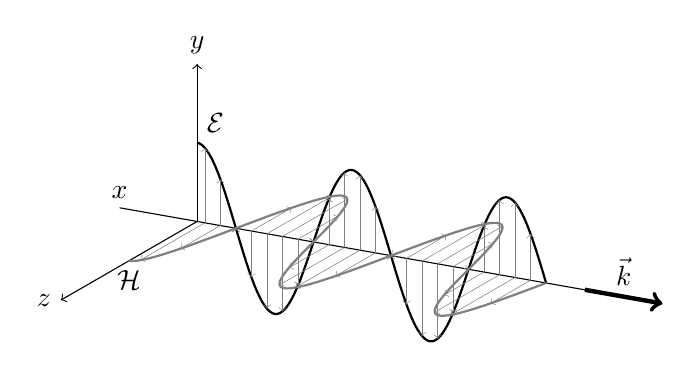
\begin{tikzpicture}[x={(-10:1cm)},y={(90:1cm)},z={(210:1cm)}]
        % Axes
        \draw (-1,0,0) node[above] {$x$} -- (5,0,0);
        \draw[->] (0,0,0) -- (0,2,0) node[above] {$y$};
        \draw[->] (0,0,0) -- (0,0,2) node[left] {$z$};
        % Propagation
        \draw[->,ultra thick] (5,0,0) -- node[above] {$\vec k$} (6,0,0);
        % Waves
        \draw[thick] plot[domain=0:4.5,samples=200] (\x,{cos(deg(pi*\x))},0);
        \draw[gray,thick] plot[domain=0:4.5,samples=200] (\x,0,{cos(deg(pi*\x))});
        % Arrows
        \foreach \x in {0.1,0.3,...,4.4} {
          \draw[->,help lines] (\x,0,0) -- (\x,{cos(deg(pi*\x))},0);
          \draw[->,help lines] (\x,0,0) -- (\x,0,{cos(deg(pi*\x))});
        }
        % Labels
        \node[above right] at (0,1,0) {$\mathcal{E}$};
        \node[below] at (0,0,1) {$\mathcal{H}$};
    \end{tikzpicture}

    \caption{Visual representation of a propagating plane wave in classical electrodynamics with $\vec k$ being the wave vector dictating the direction in which the wave propagates and is perpendicular to the wave-front \cite{Brekhovskikh1980Waves}.}
    \label{fig:em_waves}
\end{figure}

The number of oscillations per unit time is referred to as the frequency, $f$, of the field.
The quantum picture of \gls{em} fields is somewhat different.
Here, the moving charged particles are treated as ``quantum harmonic oscillators'' described via \gls{em} field tensors.

Mathematically, \gls{em} fields can be formulated within the Maxwell framework originally consisted of twenty scalar equations and subsequently reduced to four partial differential vector equations that encapsulate expressions for the relationship between fields and their sources in a symmetric form~\cite{Poljak2006Advanced}
\begin{align}
    \label{eqn:maxwell-faraday}
    \nabla \times \mathcal{E} &= -\frac{\partial \mathcal{B}}{\partial t},\\
    \label{eqn:maxwell-ampere}
    \nabla \times\mathcal{H} &= \mathcal{J} + \frac{\partial \mathcal{D}}{\partial t},\\
    \label{eqn:maxwell-gauss}
    \nabla \cdot \mathcal{D} & = \rho,\\
    \label{eqn:maxwell-gauss-magnetics}
    \nabla \cdot \mathcal{B} &= 0.
\end{align}
\Cref{eqn:maxwell-faraday} represents the differential form of the Faraday law which states that the time-varying magnetic flux density, $\mathcal{B}$, is the source of the rotating electric vector field, $\mathcal{E}$.
An extended differential formulation of the Ampere law is given in \cref{eqn:maxwell-ampere}.
It states that electric current density, $\mathcal{J}$, is the source of the rotating magnetic vector field, $\mathcal{H}$.
Furthermore, with an addition of displacement currents -- given by the time-varying electric flux density, $\mathcal{D}$, the consistency with the law of conservation of electric charge is achieved.
In \cref{eqn:maxwell-gauss}, the Gauss law, outlining the relationship between static electric fields and electric charges is given.
A static electric field points exclusively from positive towards negative charges with the net field outflow being proportional to the charge in a bounded volume of space.
On the other hand, the Gauss law for magnetism, which excludes the existence of magnetic monopoles -- the magnetic field is always solenoidal, is given in \cref{eqn:maxwell-gauss-magnetics}.

As the field propagates away from a source, it transfers
energy from its source to the surrounding space.
The general conservation of energy for a configuration consisting of electric and magnetic fields acting on charges is given by the Poynting theorem.
This theorem represents an energy balance indicating the rate of energy transfer (per unit volume) from a region of space is equal to the rate given by the work done on a charge distribution within the volume and the energy flux leaving that region reduced by the rate at which energy leaves the volume~\cite{Jackson1998Classical}.
It is written as~\cite{Durney1986Radiofrequency}
\begin{align}
    \label{eqn:poynting-theorem}
    \frac{\partial}{\partial t}\int_V \big( W_c + \frac{1}{2} \; \varepsilon \; \vec E \cdot \vec E^* + \frac{1}{2} \; \mu \; \vec H \cdot \vec H^* \big) \; \mathrm{d}V + \oint_S \big( \mathcal{E} \times \mathcal{H} \big) \; \mathrm{d} \vec S = 0.
\end{align}
In \cref{eqn:poynting-theorem}, $W_c$ represents energy of the charged particles (including both sources and losses) at a given point in the bounded volume, $V$.
Expressions $\frac{1}{2} \; \varepsilon \; \vec E^* \cdot \vec E$ and $\frac{1}{2} \; \mu \; \vec H^* \cdot \vec H$ are respectively energy stored in the electric and magnetic field, where $\varepsilon$ is the absolute permittivity and $\mu$ is the magnetic permeability.
The flow of energy through the surface, $S$, bounding the observed volume in a unit of time is defined as
\begin{align}
    \label{eqn:poynting-theorem-energy}
    \oint_S \big( \mathcal{E} \times \mathcal{H} \big) \; \mathrm{d} \vec S.
\end{align}
Within \cref{eqn:poynting-theorem-energy}, the time-varying vector field, i.e., the Ponyting vector,
\begin{align}
    \label{eqn:poynting-vector}
    \mathcal{P} = \mathcal{E} \times \mathcal{H},
\end{align}
represents the power density flow which defines the direction and amount of energy flow density at any point in space.

\section{Electromagnetic Radiation}
\gls{em} radiation is created due to periodic changes of electric and/or magnetic fields.
Depending on the periodicity and the overall \gls{em} power, different wavelengths of the \gls{em} spectrum are produced.
The frequency and wavelength are inversely proportional physical quantities whose proportionality constant is the propagation speed of \gls{em} waves in space.
In vacuum, where neither collisions nor any interaction with scatterers are captured, \gls{em} waves travel at the speed of light.
On the other hand, in lossy medium, the field travels at lower speed and can impact upon material which results in the interaction with atoms and molecules in that material.
Resulting effects depend both upon the transferred power and frequency/wavelength of the field as well as the physical properties and dimensions of the material which it interacts with.

\subsection{Non-Ionizing Electromagnetic Radiation}
With photon energy up to \SI{10}{\eV}, \gls{em} radiation is classified as non-ionizing since a single photon does not carry sufficient energy to ionize atoms or molecules by removing the most loosely bound corresponding electron.
It is grouped into different wavelength/frequency bands: \gls{uv} radiation (wavelengths of \SIrange[range-units=single,range-phrase=--]{100}{400}{\nm}), visible light (wavelengths of \SIrange[range-units=single,range-phrase=--]{400}{780}{\nm}), \gls{ir} radiation (wavelengths of \SIrange[range-units=single,range-phrase=--]{780}{1000}{\nm}), \gls{rf} \gls{em} fields (\SI{100}{\kHz} to \SI{300}{\GHz}), \gls{lf} (\SI{1}{\Hz} to \SI{100}{\kHz}) and static electric and magnetic fields.
On the other hand, even photons are electrically neutral, they still can lead to ionization of the matter indirectly through the photoelectric effect and the Compton effect.
It is generally accepted that indirectly ionizing radiation occurs for a photon's energy greater than \SI{10}{\eV} which is equivalent to the higher energy \gls{uv} part of the \gls{em} spectrum (wavelength of \SI{124}{\nm} or lower)~\cite{arpansa2022ionizing,Bulletin1999QuestionsAA}.
Thus, ionizing radiation falls into the high energy \gls{uv} spectrum, X-rays, and gamma rays.
Refer to \cref{fig:em_spectrum} for a full overview of the \gls{em} spectrum.
% source: https://tex.stackexchange.com/a/498765
\pgfdeclarehorizontalshading{visiblelight}{50bp}{% https://tex.stackexchange.com/a/348492/120853
    color(0bp)=(violet!25);
    color(8.33bp)=(blue!25);
    color(16.67bp)=(cyan!25);
    color(25bp)=(green!25);
    color(33.33bp)=(yellow!25);
    color(41.5bp)=(orange!25);
    color(50bp)=(red!25)
}%

\begin{figure}[ht]
    \centering
    \begin{tikzpicture}[%
            raylabel/.style={font=\scriptsize}
        ]
        \def\minexponent{-6}
        \def\maxexponent{6}
        \def\spectrumheight{9em}
    
        \pgfmathtruncatemacro{\nextminexponent}{\minexponent + 1}
    
        % Main foreach loop, drawing the wavelengths as powers of 10 in an alternating fashion: even on top, odd at bottom. Then connects them with help lines
        \foreach [count=\i, remember=\exponent as \previousexponent, evaluate=\i as \currentposition using int(\i/2)] \exponent in {\minexponent, \nextminexponent, ..., \maxexponent}{
            \ifodd\exponent
                \def\height{0}
            \else
                \def\height{\spectrumheight}
            \fi
    
            % Anchor at baseline to get all nodes on same baseline.
            % https://tex.stackexchange.com/questions/133227/how-to-align-text-in-tikz-nodes-by-baseline#comment300863_133227
            \node[anchor=base] (WAVELENGTH_\exponent) at (\exponent, \height) {\contour{white}{\num{e\exponent}}};
    
            \ifnum\i > 1
                \ifodd\i
                    \node (LABEL_\currentposition)
                        at ($(WAVELENGTH_\exponent)!0.5!(WAVELENGTH_\previousexponent)$)
                        {};% This is left as a node as opposed to coordinate: fill it out with '\currentposition' for debugging
                \else
                    % Do not draw connection at exponent 1:
                    \pgfmathparse{\exponent != 1}% \pgfmathparse stores result (0 or 1) in macro \pgfmathresult
                    \ifnum\pgfmathresult = 1
                        \draw[help lines]
                            (WAVELENGTH_\previousexponent) --(WAVELENGTH_\exponent)
                            node[midway] (CONNECTION_\currentposition) {}% This is left as a node as opposed to coordinate: fill it out with '\currentposition' for debugging
                            coordinate[at start] (CONNECTION_\currentposition_START)
                            coordinate[at end] (CONNECTION_\currentposition_END);
                    \fi
                \fi
            \fi
        }
    
        % Create an arrow shape that fits around all relevant nodes, but do not draw it.
        % Draw it manually later to leave out the 'bottom' of the arrow.
        % We still need this invisible arrow for lining up of coordinates
        \node[
            single arrow,
            single arrow head extend=0pt,
            single arrow tip angle=150,% Inner angle of arrow tip
            fit={([xshift=-3em]CONNECTION_1_START)(CONNECTION_1_END)(CONNECTION_\maxexponent_START)([xshift=5em]CONNECTION_\maxexponent_END)},
            inner sep=0pt
        ]
        (ARROW) {};
    
        \node[align=center] (THERM) at ([yshift=3em]WAVELENGTH_1|-ARROW.after tail) {thermal\\effects};% Only works because exponent 1 is between -1 and 3
        \draw (THERM) -| ([yshift=-1.5em]WAVELENGTH_-1|-THERM);
        \draw (THERM) -| ([yshift=-1.5em]WAVELENGTH_3|-THERM);
    
        % On background layer so already drawn arrow and scale lines cover it up nicely
        \begin{scope}[on background layer]
            \node[
                inner sep=0pt,
                outer sep=0pt,
                fit={([xshift=-2.2em]WAVELENGTH_0|-ARROW.after tail)([xshift=-2.2em]WAVELENGTH_1|-ARROW.before tail)}, shading=visiblelight]
                (SMALL_VISIBLE_LIGHT) {};
    
            \shade[
                left color=white,
                right color=violet!25,
                middle color=violet!5,
                outer sep=0pt
                ]
                (CONNECTION_3_START) -- (CONNECTION_3_END) -- ([xshift=\pgflinewidth]SMALL_VISIBLE_LIGHT.south west) -- ([xshift=\pgflinewidth]SMALL_VISIBLE_LIGHT.north west) -- cycle;
    
            \shade[
                left color=red!25,
                right color=white,
                middle color=red!5,
                outer sep=0pt,
                ]
                (CONNECTION_5_START) -- (CONNECTION_5_END) -- ([xshift=-\pgflinewidth]SMALL_VISIBLE_LIGHT.south east) -- ([xshift=-\pgflinewidth]SMALL_VISIBLE_LIGHT.north east) -- cycle;
        \end{scope}
    
        % Some labels can be drawn automatically at the designated label coordinates:
        \foreach [count=\i] \label in {
                {gamma\\rays},
                {X-rays},
                {},%Skip this one
                {\gls{ir}}
            }{
                \node[raylabel, align=center] at (LABEL_\i) {\label};
            }
    
        % These do not fit the loop and are drawn manually:
        \node[raylabel, anchor=north] at ([yshift=-3.85em]$(WAVELENGTH_-2)!0.45!(WAVELENGTH_0)$) {\gls{uv}};
    
        \node[raylabel, fill=white, align=center] at (CONNECTION_6) {\gls{rf}\\radiation};
    
        \node[raylabel, right=3em of CONNECTION_6, align=right] {\gls{lf}\\radiation};
    
        \node[raylabel, left=1em of CONNECTION_1, align=left] {cosmic\\rays};
    
        \node[
            draw,
            fill=black!20,
            below=4em of SMALL_VISIBLE_LIGHT,
            align=center,
            label=above:{\textbf{visible light}}
            ] (FULL_VISIBLE_LIGHT) {%
            \pgfspectra[width=13em,height=3em]\\%pgfspectra also has a builtin axis which of course much better than this terrible approach, but it is in nanometer
                {\SI{0.40}{} \hfill \SI{0.48}{} \hfill \SI{0.58}{} \hfill \SI{0.68}{} \hfill \SI{0.78}{\um}}
        };
    
        % Draw 'magnifying' trapeze, on background so it is covered by scale labels
        \begin{scope}[on background layer]
            \filldraw[help lines, fill=black!10] (FULL_VISIBLE_LIGHT.north east) -- (SMALL_VISIBLE_LIGHT.south east) -- (SMALL_VISIBLE_LIGHT.south west) -- (FULL_VISIBLE_LIGHT.north west) -- cycle;
        \end{scope}
    
        % Draw around arrow manually, leaving its tail open
        \draw[draw, thick] (ARROW.after tail) -- (ARROW.before head) -- (ARROW.before tip) -- (ARROW.tip) -- (ARROW.after tip) -- (ARROW.after head) -- (ARROW.before tail);
    \end{tikzpicture}
    
    \caption{Diagram of \gls{em} spectrum distribution as a function of wavelengths.}
    \label{fig:em_spectrum}
\end{figure}


By acting upon material in lossy space, non-ionizing \gls{em} waves transfer kinetic energy to surrounding bounded atoms and molecules in the material causing them to vibrate more rapidly.
This effect is accompanied by an increase in the temperature of the affected area, but it occurs only if wavelength of incident electromagnetic waves are of the same order of magnitude as the dominant dimension of the material being irradiated.
To put it in a perspective, \gls{lf} radiation has very long wavelengths (order of a thousand kilometres or more), \gls{rf} radiation have wavelengths of between \SI{1}{} and \SI{100}{\m}, with microwaves being about \SI{1}{\cm} long.
Thus, heating of biological tissue is the most prevalent in microwave spectrum and towards the lower energy part of \gls{uv} spectrum, see \cref{fig:em_spectrum}.

\subsection{Foundational Principles of Non-Ionizing Electromagnetic Radiation Effects on Tissue}
\label{sec:principles}
Conditioned by the interaction of non-ionizing radiation and biological tissue, a biological effect can be described as any biological, physical, or chemical change induced in this tissue~\cite{ICNIRP2020Principles}.
Living organisms have repair and feedback mechanisms intended primarily for preservation of homeostasis.
Once upper threshold limits in the capacity of these mechanisms are exceeded, adverse health effects may occur.
In some cases, the difference between the biological and adverse health effect is not clear as it may vary significantly upon individual's perception and sensitivity.
For this reason, adverse health effects are distinguished from other biological effects based on the World Health Organization definition of health: ``Health is a state of complete physical, mental and social well-being and not merely the absence of disease or infirmity''~\cite{WHO2022Health}.
If a biological perception appears as a consequence of non-ionizing radiation (e.g. tingling sensation~\cite{Saunders2007neurobiological}, magnetophosphenes~\cite{Lövsund1980Magnetophosphenes}, microwave hearing~\cite{Frey1962Human}), and it does not have consequences on the health of an individual, then it is not considered an adverse health effect~\cite{ICNIRP2020Principles}.

Interaction effects between non-ionizing radiation and biological tissue are roughly classified into the thermal and non-thermal category.
Low frequency \gls{rf} radiation up to \SI{100}{\kHz} usually pertains to non-thermal effects, e.g., nerve stimulation, while \gls{rf} radiation above \SI{10}{\MHz} is exclusively associated with thermal effects by means of tissue temperature rise.
The overview of the non-ionizing \gls{em} spectrum and the effects on biological tissue is outlined in \cref{tab:interaction-mechanism}.
\begin{table}[ht]
    \centering
    \caption{Summary of non-ionizing radiation effects on biological tissue.}
    \label{tab:interaction-mechanism}
    \resizebox{\textwidth}{!}{%
        \begin{tabular}{|c|c|c|}
            \hline \rowcolor[HTML]{EFEFEF}exposure to  & frequency range & \cellcolor[HTML]{EFEFEF}effect of interaction \\ \hline static magnetic fields & \SI{0}{\Hz} & induced electric fields and current \\
            \hline \gls{lf} radiation & \SI{1}{\Hz} to \SI{100}{\kHz} & stimulation of excitable cells \\
            \hline & \SI{100}{\kHz} to  \SI{10}{\MHz} & stimulation of excitable cells and tissue heating \\
            \cline{2-3} \multirow{-2}{*}{\gls{rf} radiation} & \SI{100}{\MHz} to \SI{300}{\GHz} & \\
            \cline{1-2} \gls{ir} radiation & \SI{300}{\GHz} to  $\sim$ \SI{400}{\THz} & \\
            \cline{1-2} visible light & $\sim$ \SI{400}{\THz} to  $\sim$ \SI{790}{\THz} & \\
            \cline{1-2} low energy \gls{uv} & above \SI{790}{\tera\Hz} & \multirow{-4}{*}{tissue heating} \\
            \hline
        \end{tabular}%
    }
\end{table}
Exposure to \gls{em} fields induces electric fields within tissue, which can stimulate any excitable cells of that tissue up to \SI{10}{\MHz}~\cite{Saunders2007neurobiological}.
Low frequency, pulsed \gls{em} fields of sufficient intensity may lead to the change in permeability of cell membranes and subsequent deformation of intracellular structures if the duration is shorter than the charging time of the outer membrane~\cite{Joshi2010Critical}.
Increasing the frequency, heating effects predominate and the likelihood of nerve stimulation drastically decreases.
However, evidences on the existence of non-thermal effects above \SI{100}{\MHz} exist~\cite{Romanenko2017interaction} and are usually manifested as changes in the activity of cell membranes and non-selective channels, transmembrane potentials and the cell cycle.
Since there is no scientific consensus of their adverse health effects, they fall out of the scope of this work.
It is nevertheless important to note that in~\cite{Fröhlich1968Long}, theoretical predictions of the existence of megahertz to terahertz oscillations in the living cells were postulated and have sparked great interest in risks and potentials of the interaction of external \gls{em} fields and tissues.
Biological effects at physiological levels and at cellular and molecular levels have been reviewed extensively in~\cite{Pakhomov1998Current,Zhadobov2011Millimeter}.
Authors of the latter study argue that even though there are some arguments in favor of possible interactions of high frequency \gls{em} waves, especially at \gls{mmw}, with living organisms that exclude direct and indirect thermal effects, e.g., therapeutic applications~\cite{Ziskin2006Physiological}, it is unclear if these effects can be fully explained without placing them in the thermodynamics framework.

\section{Radio-Frequency Electromagnetic Radiation Protection}
With the development and widespread deployment of electronic systems, humans are increasingly being exposed to artificial \gls{em} fields~\cite{Hirata2021Assessment}.
Most consumer electronics fall into the \gls{rf} portion of the \gls{em} spectrum as they are usually based on the services of communication and wireless transmission of information and recently, on a larger scale, on wireless power transfer.
To ensure safe use of such devices, various international bodies set guidelines or standards for limiting exposure to \gls{em} fields.
\Gls{icnirp} and \gls{ieee} International Commitee on \gls{em} Safety prescribe exposure limits through guidelines~\cite{ICNIRP2020Guidelines} and standards~\cite{IEEE2019Standard}, respectively, both for people in restricted environments and for the general public.

A high degree of protection against adverse health effects is ensured by respecting the frequency and exposure scenario dependent limits to both short- and long-term, continuous and discontinuous \gls{rf} \gls{em} fields~\cite{ICNIRP2020Guidelines,IEEE2019Standard}.
The limits are derived upon published scientific literature pertaining to the effects of \gls{rf} \gls{em} field exposure on biological systems and tissues that is classified as potentially harmful.
These limits are subsequently identified as adverse health effect thresholds~\cite{ICNIRP2020Guidelines} (or exposure limits~\cite{IEEE2019Standard}).
Additionally, reduction factors~\cite{ICNIRP2020Guidelines} (or safety margins~\cite{IEEE2019Standard}) are applied to the resultant thresholds/limits or operational threshold/limits if no direct thresholds/limits can be explicitly obtained.
Reduction factors (or safety margins) account for feature variability of individuals as well as variations in the exposure setup, environment, etc.

Now, the threshold values, incorporating reduction factors (or safety margins), are expressed in terms of \gls{br}s~\cite{ICNIRP2020Guidelines} (or \gls{drl}s~\cite{IEEE2019Standard}).
They relate to physical dosimetric quantities, either peak or averaged in time and space, that are well correlated with occurrence of harmful impact as a result of \gls{rf} \gls{em} exposure.
To facilitate the assessment of exposure in situations where the aforementioned physical quantities are difficult to measure, \gls{rl}s~\cite{ICNIRP2020Guidelines} (or \gls{erl}s~\cite{IEEE2019Standard}) are derived upon \gls{br}s (or \gls{drl}s) under worst-case exposure conditions to acquire high degree of conservatism and to provide a more-practical means of demonstrating compliance with the guidelines (or standards).

\subsection{Brief Historical Overview}
Ever since the first commercial radio station was put in operation and started broadcasting, there has been a public interest in assessment of human exposure to \gls{rf} \gls{em} radiation.
Serious endeavors in the scientific investigation of the interaction of \gls{em} waves of \gls{rf} spectrum and human tissue were initiated during the 20s of the last century given the rapidly expanded use of \gls{rf} diathermy for therapeutic tissue heating~\cite{Kovacs1945Electrotherapy}.

In the early 50s, the US Department of Defense put in operation a large number of high-power \gls{rf} transmitters to enable the advanced use of wireless communications and radar systems.
As most of the transmitters were operated in close proximity to personnel, there existed a concern about possible adverse health effects.
The Tri-Services Program (1956–1960) was put in operation and had the main goal to examine the potential impact of radiated fields on the human body~\cite{Lin1994Early}.

Although research in this area was brought to a higher level of quality~\cite{Guy1971Analyses} during the 70s, there was a growing distrust within the general population due to the increasing number of wireless electronic devices operating in the close proximity of human body whose safety was questionable due the chronic lack of concrete limits and regulations defined on the basis of rigorously verified scientific facts, but also the growing number of controversies~\cite{Foster2022Three}.
As a response, more and more computational dosimetry studies were published, mostly considering far-field exposure to plane wave radiation given the state of the technology at the time.
This culminated with publication of a series of dosimetry handbooks sponsored by the U.S. Air Force~\cite{Durney1986Radiofrequency}.

At the same time, comprehensive studies of
environmental RF fields in urban environments underwent proliferation~\cite{Tell1976Measurement}, and, to date, numerous surveys have measured environmental \gls{rf} fields from diverse technologies, e.g., \gls{rf} transmitters, base stations, mobile phones, etc., in different conditions and exposure scenarios~\cite{Jalilian2019Public}.
The first set of the formal \gls{rf} safety standards in U.S. were published during the late 60s from which the \gls{ieee} family of exposure standards, denoted C95.1-\textit{x}, where \textit{x} corresponds to the year of publication, arose.
This early limits were usually expressed in terms of the power density incident to the body and were based on canonical models predicting whole-body heating.
Subsequently, over the years, the development of international, often independent, regulatory bodies, including \gls{ansi}, \gls{icnirp}, \gls{ieee}, etc., has evolved.
Refer to~\cite{Roach2009Radiofrequency} for a more comprehensive historical background.

\Gls{icnirp}, an independent international organization, introduced generally similar guidelines; a history of the development of the organization and its guidelines are available elsewhere, e.g., in~\cite{Repacholi2017history}.
Although over the years there were significant discrepancies between \gls{ieee} C.95.1-\textit{x} standards and \gls{icnirp} guidelines, with the latest updates in 2019 and 2020, respectively, the harmonization between two sets of limits has mostly been achieved.
It is reported in~\cite{Foster2022Three} that ``a great deal since the days of the Tri-Services Program has been learned and major technical advances in exposure assessment and dosimetry have been reached''.
This includes the high-fidelity \gls{em} simulation software for computational dosimetry, large-scale, image-based libraries of 3-D human and animals models adapted to \gls{em} simulations, high-quality, commercially available instruments for accurate \gls{rf} exposure assessment, etc.

During the last decade, research has at least doubled on all fronts: from experimental to epidemiological to dosimetric/technical studies.
However, the greatest progress can be seen in the quality and number of published studies carried out in computational dosimetry research, the main idea of which is the realization of precise simulations at high frequencies in the near field~\cite{Diao2021Effect}.
In 2021, in total $N = $ 375 studies related to computational dosimetry have been published concerning the exposure to \gls{rf} \gls{em} waves and/or mobile communications in general (see \cref{fig:research_compilation_2021}), which is more than a double compared to the number of published experimental studies ($N = $ 140).
\begin{figure}[ht]
    \centering
    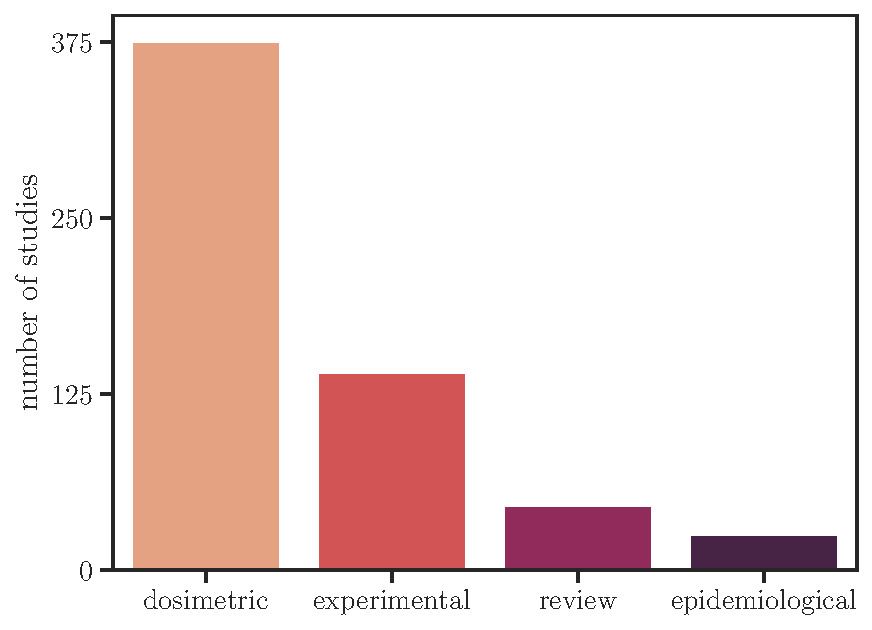
\includegraphics[width=0.8\textwidth]{artwork/research_compilation_2021.pdf}
    \caption{Papers published in 2021 related to research on bioeffects of \gls{rf} fields and/or mobile communications. Compiled from the database of publications at \url{emf-portal.org}.}
    \label{fig:research_compilation_2021}
\end{figure}
The reason for this is the market breakthrough of new wireless communication devices, primarily based on the \gls{5g} cellular technology, which, in addition to utilization of higher parts of the \gls{rf} spectrum compared to preceding generations, employs \gls{mimo} antennas and beam-steering~\cite{Andrews2014What}.
Considering the hard-to-maintain control conditions of the laboratory and expensive equipment, especially at \gls{mmw}, there is a dearth of accurately assessed and adequate experimental data.
The available experimental studies do not provide sufficient information for a meaningful safety assessment~\cite{Simkó20195G}.
Additionally, the advent of numerical methods~\cite{Poljak2018On}, e.g., \gls{fdtd}, \gls{fem}, \gls{bem}, \gls{mom}, etc., computing power and its overall availability, facilitated by the publicly available, highly-accurate databases on the dielectric properties of numerous human and animal tissues~\cite{Gabriel1996Compilation} has enabled progress in computer dosimetry and computational bioelectromagnetics in general.
The evolution of research from 1950 to 2021 in the field of \gls{rf} and/or mobile communications exposure assessment and dosimetry is visualized in \cref{fig:research_compilation}.
\begin{figure}[ht]
    \centering
    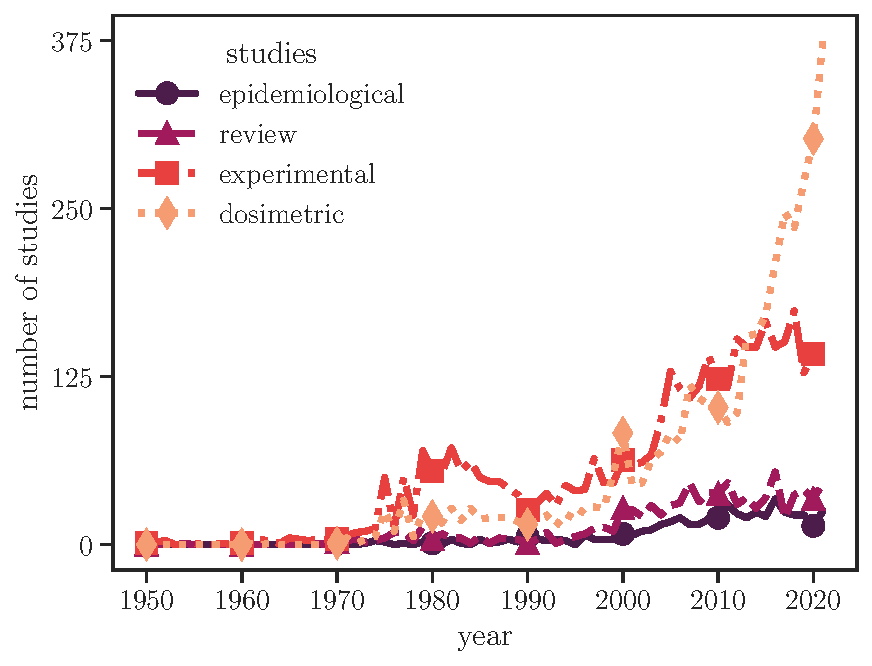
\includegraphics[width=0.8\textwidth]{artwork/research_compilation.pdf}
    \caption{Papers published over years from 1950 to 2021 related to research on bioeffects of RF fields and/or mobile communications. Compiled from the database of publications at \url{emf-portal.org}.}
    \label{fig:research_compilation}
\end{figure}

\subsection{Scientific Basis for Limiting Radio-Frequency Exposure}
As pointed out in the previous section, the main component of absorbed \gls{em} fields inside the body is the electric field.
Below \SI{10}{\MHz}, induced electric fields may stimulate nerves and, in rare occasions, cause dielectric breakdown of biological membranes~\cite{Swicord2008Has}.
Such and similar effects are defined as non-thermal and can be classified into four groups: resonance mechanisms, coupling with non linear systems, effects due to the direct action of electric and magnetic fields, and cooperative mechanisms due to interactions among several membrane components~\cite{DInzeo200dDeliverable}.
Above \SI{100}{\kHz}, the result of the interaction between induced electric fields and polar molecules or free charges within the exposed body is the kinetic energy.
It makes the polar molecules to rotate and oscillate around their center, while charges to form the electric current.
Increased kinetic energy leads to more frequent interaction with other polar molecules and charged particles, which ultimately causes conversion of kinetic into thermal energy~\cite{Foster2018Modeling}.

In order to evaluate the heating effects, it is important to quantify the absorbed \gls{em} power within exposed tissue.
It is generally considered that below \SI{6}{\GHz}, \gls{em} fields penetrate deep, whereas above this frequency, the power is dissipated mostly across the surface of the exposed tissue~\cite{Ziskin2018Tissue}.
The power transmission coefficient and power penetration depth into the uniform half plane of tissue with dielectric properties of dry skin as frequency-dependent functions are shown in \cref{fig:penetration_depth}.
\begin{figure}[ht]
    \centering
    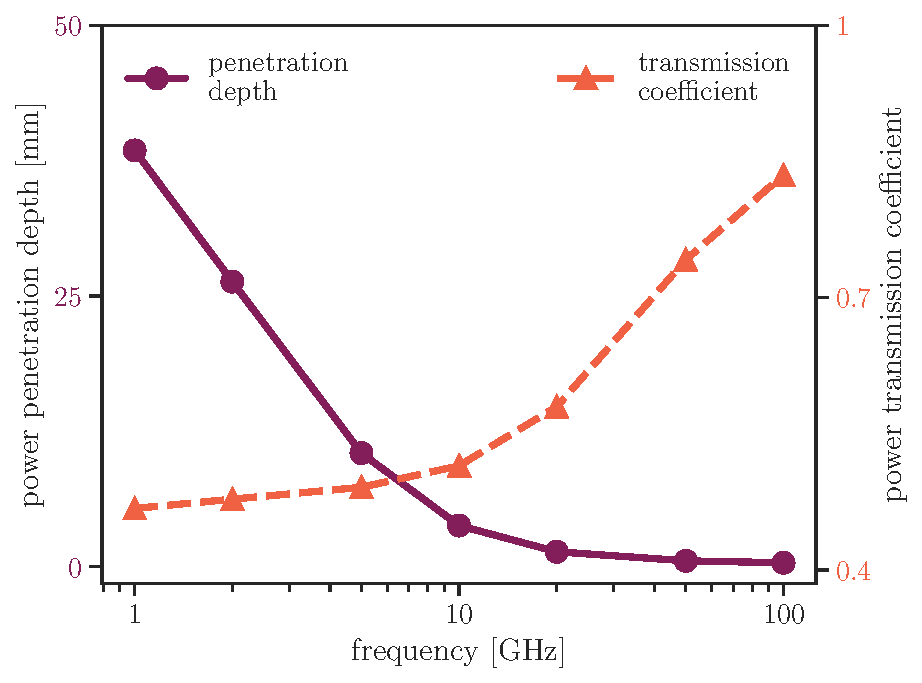
\includegraphics[width=0.8\textwidth]{artwork/penetration_depth.pdf}
    \caption{Power transmission coefficient and power penetration depth into dry skin as functions of frequency.}
    \label{fig:penetration_depth}
\end{figure}
Dielectric properties of dry skin are taken from~\cite{Gabriel1996Compilation}.
Power penetration depth into the tissue is defined
as the distance beneath the surface at which the power density has fallen to a factor of $1/e$ below that at the surface -- one-half of the more commonly reported wave penetration depth~\cite{Foster2016Thermal}.

Both guidelines and standards set (operational) threshold levels to restrict temperature rise rather than absolute temperature as it is dependent on many factors that are not conditioned by exposure to \gls{rf} \gls{em} fields.
Such factors, e.g., sex, age, thermoregulation, that are subject to inter-individual features together with additional confounding variables as surrounding temperature, clothing, and work rate are out of the scope of guidelines/standards.

Temperature rise can be further differentiated to steady-state and brief temperature rise.
Steady-state temperature rise allows time for heat to dissipate over a larger tissue mass and for thermoregulatory processes to become active.
Steady-state rise of body core temperature is generally limited to \SI{1}{\celsius} although there are no scientific evidences of adverse health effects in the event of even greater temperature increase.
Due to the limited literature available, steady-state temperature rise of \SI{1}{\celsius} has been adopted in a conservative manner as it triggers significant physiological changes, e.g., thermoregulatory responses~\cite{Heuvel2017independent} which are not represented as adverse health effects.

Additionally, steady-state local temperature rise is defined to account for specific exposed body regions such as the head and torso, or limbs.
It is accepted that local temperature rise should be limited to \SI{5}{\celsius} for regions  containing tissue with normothermal temperature in the \SIrange[range-units=single,range-phrase=--]{33}{36}{\celsius} range.
For regions with higher normothermal temperature in the \SIrange[range-units=single,range-phrase=--]{36}{38.5}{\celsius} range, e.g., tissues in the head, eyes, abdomen, thorax, pelvis, etc., local temperature rise should be limited to \SI{2}{\celsius}.
These limits are based on the experimental human studies~\cite{Walters2000Heating} given the fact that damage may occur at tissue temperature of \SIrange[range-units=single,range-phrase=--]{41}{43}{\celsius}~\cite{Dewhirst2003Basic} with the likelihood and severity of damage increasing with the increase of exposure time~\cite{ICNIRP2020Guidelines}.

Finally, rapid temperature rise can result in heterogeneous temperature distribution over mass or surface of the exposed tissue before thermoregulatory responses become active that allow heat dissipation within the tissue~\cite{Foster2016Thermal,Foster2017Thermal,Laakso2017Human,Kodera2018Brief}. This will be discussed in more detail in the following sections.

\subsection{Basic Restrictions}
\Gls{br}s/\gls{drl}s (from now on in the text only ``\gls{br}'' abbreviation will be used for the sake of brevity and improved readibility) have been derived from the levels of \gls{rf} \gls{em} fields that correspond to the (operational) adverse health effects.
Typically, \gls{br}s concerning \gls{rf} \gls{em} fields are frequency dependent dosimetric quantities that are treated separately depending on the spatio-temporal scale of exposure.

For steady-state body core temperature rise, whole-body average \gls{sar} is defined as the \gls{br} at \SI{100}{\kHz} to \SI{300}{\GHz}.
\Gls{sar} represents the rate at which energy is absorbed per unit mass by a human body when exposed to \gls{rf} \gls{em} fields.
It is defined as the power absorbed per mass of tissue and has units of \SI{}{\watt\per\kg}.
Theoretical modeling and generalization from experimental research across a range of different species led both \gls{icnirp} and \gls{ieee} to set whole-body average \gls{sar} of \SI{4}{\watt\per\kg}, averaged over the entire body mass and a 30-minute interval as the exposure level corresponding to the operational adverse health effect threshold for an increase in body core temperature of \SI{1}{\celsius}.
Additional reduction/safety factor of 10 is applied subsequently to account for scientific uncertainty and inter-variability in thermal physiology of exposed occupational workers.
Furthermore, a reduction factor of 50 is applied for general public.

\Gls{sar} spatially averaged over \SI{10}{\g} provides an appropriate proxy for the local steady-state temperature rise of the tissue exposed to \gls{rf} \gls{em} waves at \SI{100}{\kHz} to \SI{6}{\GHz}.
A somewhat arbitrary mass of \SI{10}{\g} is used as heat diffusion rapidly distributes the thermal energy to a much larger volume even though the distribution of temperature can initially be heterogeneous~\cite{Hirata2009correlation}.
For head and torso, \gls{sar} of \SI{20}{\watt\per\kg} averaged over \SI{10}{\g} and 6-min interval is identified to correspond well to the (operational) adverse health effect threshold.
Again, safety factor of 2 is applied for occupational exposure and 10 for the general public.
On the other hand, limbs are composed of tissues with the generally lower normothermal temperatures.
Thus, \gls{sar} of \SI{40}{\watt\per\kg} averaged over \SI{10}{\g} and 6-min interval is set as the \gls{br} in this case.
Reduction factors match those for the head and torso, again to account for scientific uncertainty and inter-individual features of exposed individuals both in occupational exposure and in the general public.

At higher frequencies, around \SI{90}{\percent} of the total \gls{em} power is dissipated within first (few) \SI{}{mm} of the exposed tissue (\SI{8}{\mm} at \SI{6}{\GHz} and \SI{0.81}{\mm} at \SI{30}{\GHz}~\cite{Sasaki2017Monte}), see \cref{fig:sar_decay}.
\begin{figure}[ht]
    \centering
    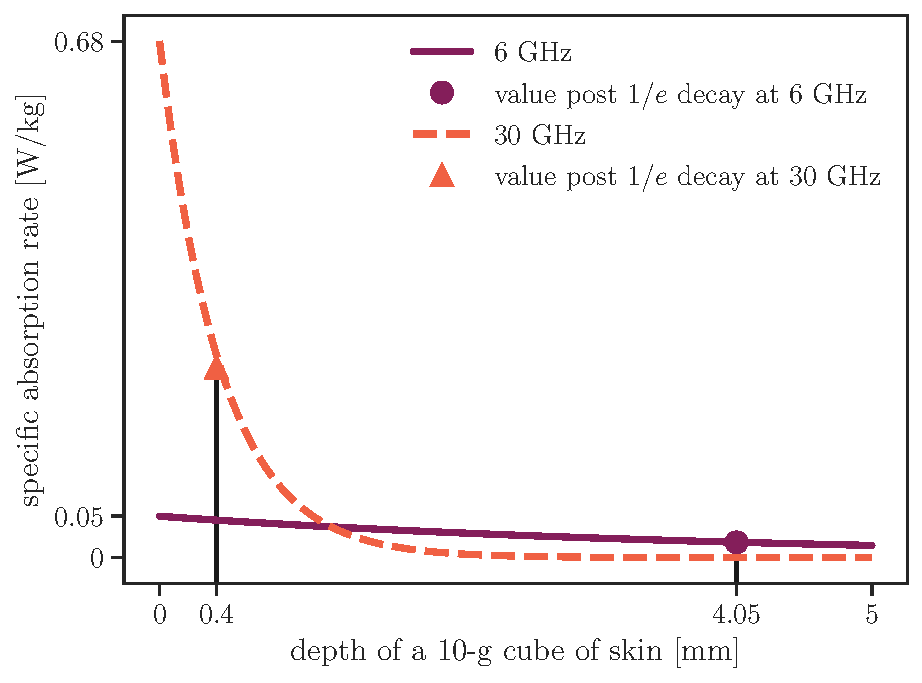
\includegraphics[width=0.8\textwidth]{artwork/sar_decay.pdf}
    \caption{Specific absorption rate as a function of depth into the homogeneous block of tissue with dielectric properties of dry skin. It is assumed that the model is exposed by a plane wave with power density of \SI{1000}{\watt\per\meter\squared}.}
    \label{fig:sar_decay}
\end{figure}
Thus, it is more appropriate to describe absorbed power over surface area.
At \SI{6}{\GHz}, \gls{br} for local exposure are expressed by means of the \gls{apd} as the most of the power is absorbed in the upper portion of a 10-g \gls{sar} cubic volume.
For dry skin of the average density of \SI{1109}{\kg\per\m\cubed}, the cube volume corresponds to \SI{2.15}{\cm\cubed}.
Recent thermal modeling~\cite{Hashimoto2017On} and analytical studies~\cite{Foster2017Thermal} suggest that at the \SIrange[range-units=single,range-phrase=--]{6}{30}{\GHz} range, the exposure over a square averaging area of \SI{4}{\cm\squared}, which matches the area of the front surface of 10-g cube, provides a good correlation for local maximum temperature rise.
This is further supported by simulations of realistic exposure scenarios~\cite{He2018RF}.
To account for narrow beam formation at higher frequencies, the \gls{apd} should be computed on the most exposed area of \SI{1}{\cm\squared} at the \SIrange[range-units=single,range-phrase=--]{30}{300}{\GHz} range.
This ensures that the operational adverse health effect thresholds are not exceeded over smaller regions provided that it does not exceed 2 times the value for the averaging area of \SI{4}{\cm\squared}~\cite{Foster2016Thermal}.
The \gls{apd} of \SI{200}{\W\per\m\squared} averaged over 6-min interval and \SI{4}{\cm\squared} surface area of the exposed region on the body corresponds to the operational adverse health effect threshold for bot the head/torso and limb region.
As with \gls{sar}, a factor of either 2 or 10 is additionally applied as a precautionary measure for occupational exposure or the general public, respectively.

\Gls{br}s for rapid temperature rise after a brief exposure are defined by means of the \gls{sa} at the \SI{400}{\MHz} to \SI{6}{\GHz} range as a function of time.
Much like \gls{sar}, \gls{sa} is spatially averaged over a 10-g cubic mass.
Concrete formulations and values are available elsewhere, e.g. in~\cite{ICNIRP2020Guidelines,IEEE2019Standard}.
An additional safety factor of 2 or 10 is applied to \gls{sa} for occupational exposure or the general public, respectively, to account for scientific uncertainty as well as variability of environmental conditions, physical activity levels, and thermal physiology across the population.

Above \SI{6}{\GHz}, following the same reasoning as for the case of setting \gls{br}s for local steady-state temperature rise, the absorbed energy density is averaged over a square \SI{4}{\cm\squared} area of the most exposed body region of interest.
To account for focal beam exposure at the \SIrange[range-units=single,range-phrase=--]{30}{300}{\GHz} range, averaging should be performed additionally over a square \SI{1}{\cm\squared} area whereas the absorbed energy density should be at most twice the value for a square \SI{1}{\cm\squared} averaging area.
Again, safety factors of 2 and 10 are respectively applied for occupational exposure and the general public, respectively.

\subsection{Exposure Reference Levels}
\Gls{rl}s/\gls{erl}s (from now on in the text only ``\gls{rl}'' abbreviation will be used for the sake of brevity and improved readability) have been derived from a combination of computational and measurement studies to provide more practical means of demonstrating compliance using physical quantities that are easy to assess without the need of having a human body in the measurement loop.
The measurement takes place in free space, where instead of absorbed, incident values are taken into consideration.
In the relevant literature, the term ``exposure assessment'' refers to the evaluation of the level of \gls{rf} \gls{em} energy incident on the exposed body, while ``dosimetry'' refers to determining the absorption of \gls{rf} \gls{em} energy within that body~\cite{Chou1996Radio}.
As incident fields do not undergo any losses caused by the interaction with the body, \gls{rl}s are always more conservative in practice than the corresponding \gls{br}.

The quantities used for specifying \gls{rl} are the \gls{Einc}, \gls{Hinc}, \gls{ipd}, plane-wave equivalent \gls{ipd}, \gls{Uinc}, and \gls{Ueq}, measured outside the body, and electric current inside the body.
Important to consider is to how well the aforementioned physical quantities serve to predict the corresponding physical quantities used to assess compliance with the \gls{br}s.
The accuracy of predictions is strongly related to whether external \gls{em} fields can be considered to be within the far-field, radiative near-field or reactive near-field zone.
Additional confounding variables are the frequency, physical dimensions of the source of external \gls{em} fields, separation distance between the source and body, etc.
Taking all this into consideration, both the \gls{icnirp} guidelines~\cite{ICNIRP2020Guidelines} and \gls{ieee} standard~\cite{IEEE2019Standard} have more conservative, but slightly different rules for exposure in the reactive and near-field than far-field zone~\cite{Hirata2020Difference}.

In this work, the emphasis is the exposure to \gls{rf} \gls{em} waves at the \SIrange[range-units=single,range-phrase=--]{6}{300}{\GHz} range, details for determination of \gls{rl}s out of this range can be found elsewhere, e.g., in chapter ``Reference levels'' of \gls{icnirp}'s 2020 guidelines~\cite{ICNIRP2020Guidelines} and chapter 4.3 ``\gls{drl}s and \gls{erl}s for exposure to electromagnetic fields -- Thermal effects (\SI{100}{\kHz} to \SI{300}{\GHz})'' in the \gls{ieee} C95.1-2019 standard~\cite{IEEE2019Standard}.
At the \SIrange[range-units=single,range-phrase=--]{6}{300}{\GHz} range, the \gls{ipd} is defined as the \gls{rl} averaged during 6-min interval for local exposure either as peak value (at \SI{6}{\GHz}) or spatially-averaged over any exposed \SI{4}{\cm\squared} area in the shape of square (above \SI{6}{\GHz}).
Additionally, at and above \SI{30}{\GHz}, the \gls{ipd} must be averaged over a square \SI{1}{\cm\squared} projected body surface with the restriction it cannot be twice as large compared to the corresponding \SI{4}{\cm\squared} area.

At \SI{6}{\GHz}, within the far-field zone, compliance is demonstrated if the peak spatial \gls{ipd} does not exceed prescribed value.
The plane-wave equivalent \gls{ipd} can be used to substitute the peak spatial \gls{ipd} when appropriate.
Within the radiative near-field zone, compliance is assessed only by using thepeak spatial \gls{ipd}.
Finally, in the reactive near-field zone, \gls{rl}s cannot be used to demonstrate compliance -- \gls{br}s must be assessed in this case.
The same logic applies above \SI{6}{\GHz} and up to \SI{300}{\GHz} where instead of the peak spatial value, the spatially averaged \gls{ipd} is used to demonstrate compliance with prescribed limits.
A detailed overview of \gls{rl} for local exposure, averaged over 6-min interval at the \SIrange[range-units=single,range-phrase=--]{6}{300}{\GHz} range can be found in \cref{tab:rls}.
\begin{table}[ht]
\begin{center}
\caption{(Exposure) reference levels averaged over 6-min interval at the \SIrange[range-units=single,range-phrase=--]{6}{300}{\GHz} range.}
\label{tab:rls}
\resizebox{\textwidth}{!}{%
\begin{tabular}{|c|c|c|cc|}
\hline
\cellcolor[HTML]{EFEFEF} & \cellcolor[HTML]{EFEFEF} & \cellcolor[HTML]{EFEFEF} & \multicolumn{2}{c|}{\cellcolor[HTML]{EFEFEF}{\color[HTML]{333333} value${}^{*}$ [\SI{}{\watt\per\m\squared}]}} \\ \cline{4-5} 
\multirow{-2}{*}{\cellcolor[HTML]{EFEFEF}\begin{tabular}[c]{@{}c@{}}exposure\\ scenario\end{tabular}} & \multirow{-2}{*}{\cellcolor[HTML]{EFEFEF}frequency [GHz]} & \multirow{-2}{*}{\cellcolor[HTML]{EFEFEF}\begin{tabular}[c]{@{}c@{}}(exposure)\\ reference levels\end{tabular}} & \multicolumn{1}{c|}{ICNIRP~\cite{ICNIRP2020Guidelines}} & IEEE~\cite{IEEE2019Standard} \\ \hline
 & 6 &  & \multicolumn{1}{c|}{200} & 200 \\ \cline{2-2} \cline{4-5} 
 & 6--300 &  & \multicolumn{1}{c|}{$275 \; f_G^{-0.177}$} & $274.8 \; f_G^{-0.177}$ \\ \cline{2-2} \cline{4-5} 
\multirow{-3}{*}{\begin{tabular}[c]{@{}c@{}}occupational\\ (restricted\\ environments)\end{tabular}} & 300 &  & \multicolumn{1}{c|}{100} & 100 \\ \cline{1-2} \cline{4-5} 
 & 6 &  & \multicolumn{1}{c|}{40} & 40 \\ \cline{2-2} \cline{4-5} 
 & 6--300 &  & \multicolumn{1}{c|}{$55 \; f_G^{-0.177}$} & $55 \; f_G^{-0.177}$ \\ \cline{2-2} \cline{4-5} 
\multirow{-3}{*}{\begin{tabular}[c]{@{}c@{}}general public\\ (unrestricted\\ environment)\end{tabular}} & 300 & \multirow{-6}{*}{\gls{ipd}} & \multicolumn{1}{c|}{20} & 20 \\ \hline
\end{tabular}%
}
\end{center}
${}^{*}f_G$ stands for the frequency in \SI{}{\GHz}.
\end{table}

Furthermore, to put values in the visual frame of reference, in \cref{fig:reference_levels}, the \gls{ipd} as a function of frequency is shown over the \SIrange[range-units=single,range-phrase=--]{6}{300}{\GHz} range.
\begin{figure}[ht]
    \centering
    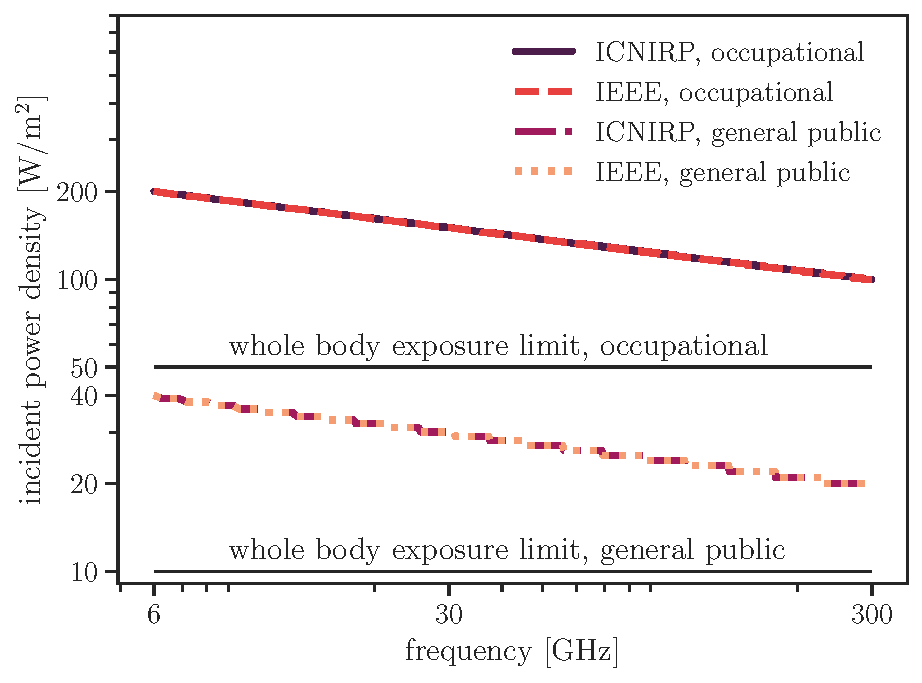
\includegraphics[width=0.8\textwidth]{artwork/reference_levels.pdf}
    \caption{Reference levels for occupational exposure and general public averaged over 6-min interval at the \SIrange[range-units=single,range-phrase=--]{6}{300}{\GHz} range. Both \gls{icnirp} and \gls{ieee} curves for the \gls{ipd} as a function of the frequency are shown to demonstrate harmonization between prescribed limits. Additionally, black horizontal lines show (exposure) reference levels for whole body exposure over 30-min interval at constant values of \SI{10}{\watt\per\m\squared} and \SI{50}{\watt\per\m\squared} for general public and occupational exposure, respectively.}
    \label{fig:reference_levels}
\end{figure}
\Gls{rl}r for whole-body exposure are also shown both for occupational exposure and general public and are set to constant values of \SI{50}{} and \SI{10}{\watt\per\m\squared}, respectively.
As for local exposure, at \SI{6}{\GHz} within the far-field zone, compliance is demonstrated if the peak spatial \gls{ipd} does not exceed the prescribed value where, if appropriate, the plane-wave equivalent \gls{ipd} can be used instead of the \gls{ipd}.
In the radiative near-field zone, compliance is demonstrate only if the \gls{ipd} does not exceed the limits.
Finally, within the reactive near-field zone, compliance cannot be demonstrated by using the \gls{ipd} and the corresponding dosimetric value must be assessed.

In cases of simultaneous exposure to multiple frequency \gls{rf} \gls{em} fields, it is important to evaluate whether these exposures are additive in their effect.
This cumulative effect should be treated separately for the thermal and electrical stimulation, and restrictions should be set accordingly.
This issue is out of the scope of this document.
Details can be found elsewhere, e.g., in~\cite{ICNIRP2020Guidelines, IEEE2019Standard}.
However, it is noteworthy that in~\cite{Miura2021Power}, simultaneous exposure is evaluated at \SI{2}{} and \SI{28}{\GHz} by evaluating power absorption and skin temperature rise in the near-field zone of realistic antenna models.
It is demonstrated that the effect of superposition is marginal in all cases except when the patch antenna array and inverted-F antenna are separated by less than \SI{50}{\mm} at \SI{5}{\mm} antenna-body separation.


% chapter 3 
\clearpage
\chapter{Exposure Assessment and Dosimetry in the Era of 5G}
\label{chap:methods}

\section{Specific Absorption Rate}
Generally, heating effects are correlated well with the amount of \gls{em} field power absorbed by biological tissue.
The total power absorbed per unit mass is given in terms of \gls{sar} which is measured in \SI{}{\watt\per\kg}.
According to~\cite{Foster2022Three}, the first mention of the term ``\gls{sar}'' is found in 1975 PhD dissertation by Chou~\cite{Chou1975Effects}.

Mathematically, \gls{sar} represents the rate of change at which \gls{em} energy is absorbed by or dissipated in a unit mass, contained in a volume element:
\begin{align}
    \label{eqn:sar_1}
    \text{SAR} = \frac{\partial}{\partial t} \Big( \frac{\partial W}{\partial m} \Big).
\end{align}
If exposed tissue has a constant density, $\rho$, the above expression can be written as
\begin{align}
    \label{eqn:sar_2}
    \text{SAR} = \frac{\partial}{\partial t} \Big( \frac{\partial W}{\rho \; \partial V} \Big),
\end{align}
where $V$ is a volume element of interest.
In dielectric sense, any biological tissue can be described as lossy, magnetically transparent material characterized by the frequency dependent relative complex dielectric permittivity,  $\varepsilon^*$, and relative permeability, $\mu_r = 1$~\cite{Sasaki2014Measurement}.
Therefore, in practical situations, \gls{sar} can be assessed by using the following expression:
\begin{align}
    \label{eqn:sar_3}
    \text{SAR} = \frac{\sigma \; |\mathbf{E}|^2}{\rho},
\end{align}
where $\sigma$ represents the conductivity of tissue measured in \SI{}{\siemens\per\m}, and $\mathbf{E}$ is the \gls{rms} value of the electric field at a single point within tissue.

Temperature rise of the exposed tissue is shown to be strongly correlated with the value of \gls{sar}, and in the case of brief \gls{em} exposure where heat loss is not significant, it can be approximated as
\begin{align}
    \label{eqn:sar_4}
    \text{SAR} = C \; \frac{\partial T}{\partial t},
\end{align}
where $C$ is specific heat capacity expressed in \SI{}{\joule\per\kg\per\celsius}, and $T$ is temperature in \SI{}{\celsius}.
However, in realistic exposure scenarios that are neither brief nor can be treated by homogeneous models, heat loss is significant as a large amount of heat rapidly diffuses due to active thermoregulatory mechanism.
For this reason, \gls{sar}, as a proxy for temperature rise, must be averaged over either whole body, or, in the case of local exposure, 10-g equivalent of tissue volume~\cite{McIntosh2011SAR}.
Spatially-averaged \gls{sar} over \SI{10}{g} has been shown to approximate temperature rise well up to \SI{6}{\GHz} for both the homogeneous cubical and morphologically accurate body model~\cite{Hirata2009correlation}.
Additionally, in cases where simplistic tissue models are utilized, peak-spatial \gls{sar} can also be used to correlate temperature rise at lower frequencies, concretely \SI{150}{}, \SI{400}{} and \SI{900}{\MHz} bands, which is confirmed by considering a 3-D realistic human body model~\cite{Hirata2006Correlation}.
At higher frequencies, especially above \SI{6}{\GHz}, the same cannot be stated as the correlation between peak-spatial \gls{sar} and maximum temperature rise is at most modest for realistic exposure of morphologically accurate body models~\cite{Morimoto2016Relationship}.

Whole-body exposure is accompanied with the assessment of whole-body average \gls{sar}, which is dependent on the spatial distribution of the internal electric field, electric conductivity of tissue, and tissue density.
Taking all this into account, whole-body averaged \gls{sar} is defined as the ratio of the total power absorbed in the whole body and the whole body mass:
\begin{align}
    \label{eqn:sar_wb}
    \text{whole-body SAR} = \frac{\int_{V_\text{wb}} \sigma \; |\mathbf{E}|^2 \; \mathrm{d}V}{\int_{V_\text{wb}} \rho \; \mathrm{d}V},
\end{align}
where $V_\text{wb}$ is the volume of the exposed body.

Different averaging schemes and masses have been numerically analyzed in terms of how well they predict local temperature rise~\cite{Hirata2009correlation,McIntosh2011SAR}.
It is generally accepted that a cubic averaging mass of \SI{10}{\g}, including all tissues, serves as an appropriate spatial averaging volume equivalent up to \SI{6}{\GHz}.
Furthermore, it is important to note that 10-g volume corresponds to approximately \SI{2.15}{\cm\cubed} cube assuming that the density of exposed tissue is the same as that of water, i.e., \SI{1000}{\kg\per\m\cubed}.

On average, the time required to reach a steady state for the case of the whole body exposure is 30 minutes or more, while for the local exposure an interval of 6 minutes is considered to be sufficient.
The reasoning behind the temporal averaging consideration in the case of the whole body is based on analytical approximations as presented in ``Appendix A'' in the \gls{icnirp} guidelines~\cite{ICNIRP2020Guidelines}, but also on experimental studies, e.g.,~\cite{Hirata2008FDTD,Nelson2013High}.
The time constant is governed by the rate of exchange of heat between the core of the body and the surrounding environment~\cite{Adair2003Thermoregulatory}.
On the other hand, the matter of temporal averaging for local exposure is somewhat more complex as it depends on two distinct factors which are as follows: the rate of convective heat exchange by blood flow, and conduction of heat from the exposed area~\cite{Foster2017Thermal}.
Both simple analytical models~\cite{Foster2017Thermal} and detailed numerical analysis~\cite{Morimoto2017Time} demonstrate that the overall rate of heat dissipation from an exposed region depends mostly on thermal convection by blood flow.
In turn, thermal convection depends on multiple factors, but is generally accepted that the 6-min interval allows for reaching steady-state in most exposure scenarios.

\section{Transition to Power Density}
Previously, in 1998 version of the \gls{icnirp} guidelines~\cite{ICNIRP1998Guidlines}, \gls{sar} was used up to \SI{10}{\GHz}, whereas the power density was used above this transition frequency.
Conversely, in 2005 version of the \gls{ieee} standard~\cite{IEEE2005Standard}, the transition frequency was set to \SI{3}{\GHz}.
The said discrepancy caused a discontinuity in the exposure limits across the transition frequency~\cite{Colombi2015}.
In recent literature, it has been shown that at \SI{6}{\GHz} and especially at \gls{mmw}, \gls{sar} no longer represents an appropriate surrogate for local temperature rise.
This is mainly because at such high frequency, \gls{em} energy is deposited predominantly in superficial tissues, i.e., cutaneous tissue~\cite{Ziskin2018Tissue,Zhadobov2011Millimeter}.
With an increase in frequency, the penetration depth of the impinging \gls{em} wave decreases, and it leads to more superficial distribution of \gls{em} energy which is additionally influenced by dielectric properties of tissue (also frequency-dependent).
Therefore, the power density absorbed in the skin provides a better approximation of maximum temperature rise on the surface of the exposed body at the \SIrange[range-units=single,range-phrase=--]{6}{300}{\GHz} range~\cite{Funahashi2018Area-Averaged}.
The break-point between volume-averaged \gls{sar} and surface-averaged power density and the need of harmonization between the two sets of exposure limits date back to 2011~\cite{McIntosh2011SAR}.
In this paper, authors argue that even though combined results of a simple planar and complex body modeling did not provide a clear indication of which of the two metrics was better correlated with induced temperature rise from \gls{rf} heating between \SI{3}{} and \SI{10}{\GHz}, from a practical point of view, \SI{6}{\GHz} was shown to result with the greater ease of the assessment of the spatially-averaged power density compared to volume-averaged \gls{sar}.
Considering this work, and more recent analytical~\cite{Foster2016Thermal,Foster2017Thermal,Ziskin2018Tissue} and numerical studies~\cite{Hirata2019Setting}, in recent updates of the \gls{icnirp} guidelines and \gls{ieee} standard, transition frequency is set to \SI{6}{\GHz} which led to the final harmonization between the two sets of limits.

\section{Absorbed Power Density}
\subsection{Definitions}
As stated in the previous section, the power density absorbed in the tissue undergoes exponential decay from the surface to deeper regions:
\begin{align}
    \label{eqn:apd}
    S_\text{ab} = S(z=0) \; \int_{z=0}^{z_\text{max}} \exp{ \Big(- \frac{2z}{\delta} \Big)} \; \mathrm{d}z,  
\end{align}
where $S_\text{ab}$ stands for the \gls{apd} spatially averaged on the tissue surface, $S(z=0)$ stands for the specific \gls{apd} averaged on the exposed surface, i.e., at $z=0$, $\delta$ is the penetration depth perpendicular into the tissue ($z$-direction in this case), $z_\text{max}$ is the depth of the exposed tissue which must be sufficiently large to compensate for $\delta$.
The specific \gls{apd} at $z=0$, averaged over an area $A$ can be written as
\begin{align}
    \label{eqn:specific_apd}
    S(z=0) = \frac{1}{A} \; \iint_A \rho(x, y, 0) \; \text{SAR}(x, y, 0) \; \mathrm{d}x \mathrm{d}y.
\end{align}
To demonstrate the exponential decay phenomenon, consider the following example.
For 1000 values sampled from a continuous uniform distribution bounded within the \SI{0}{\watt\per\m\squared} and the maximum permissible incident power density at \SIlist[list-units=single]{10;30;60;100}{\GHz}, the mean and standard deviation are calculated.
The specific \gls{apd} is then approximated by using the following expression:
\begin{align}
    \label{eqn:specific_apd_approx}
    S(z=0) = T \cdot \text{IPD},
\end{align}
where $T$ is transmittance defined as
\begin{align}
    \label{eqn:transmittance}
    T = 1 - |\Gamma|^2,
\end{align}
and where $\Gamma$ is the reflection coefficient derived from the dielectric properties of the tissue, shape of the body surface, incident angle and polarization.
In this case, plane wave with normal incidence onto the planar homogeneous dry skin half-space is considered.
Dielectric properties are defined via relative complex permittivity~\cite{Wu2015human},
\begin{align}
    \label{eqn:rel_complex_permittivity}
    \varepsilon^* = \varepsilon' + j \; \varepsilon'',
\end{align}
where
\begin{align}
    \varepsilon'' = \frac{\sigma}{2 \pi f \varepsilon_0}.
\end{align}
and $\varepsilon'$ is extracted from~\cite{Gabriel1996Compilation} at corresponding $f$. 
This sampling procedure is then repeated 1000 times to obtain the actual expected specific \gls{apd} within the interval of values that can be obtained given the range of \gls{ipd}s.
In \cref{fig:pd_decay}, the intensity of the power density at $z=\SI{0}{\mm}$ is shown with full line, whereas the value of the  power density absorbed at $z=\SI{1}{\mm}$ depth-wise into the dry skin is shown by using dashed line.
\begin{figure}[ht]
    \centering
    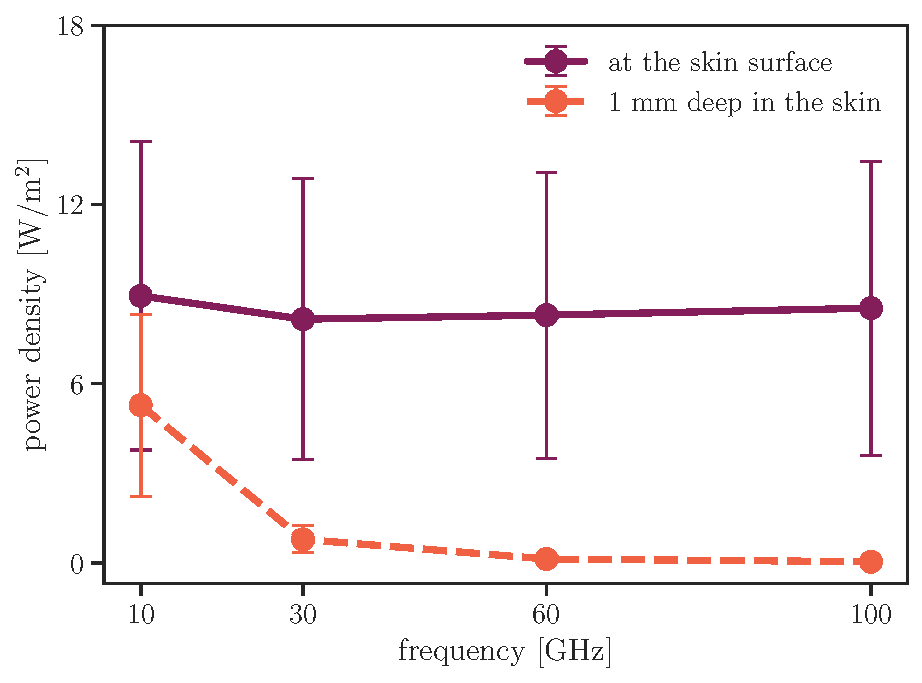
\includegraphics[width=0.8\textwidth]{artwork/pd_decay.pdf}
    \caption{Power density as a function of frequency. At the skin surface (full line), it stays constant with an increase in frequency given the incident power density is bounded between \SI{0}{\watt\per\m\squared} and maximum permissible value as prescribed in~\cite{ICNIRP2020Guidelines,IEEE2019Standard}. At \SI{1}{\mm} depth, power density undergoes steep exponential decay with an increase in frequency.}
    \label{fig:pd_decay}
\end{figure}
With an increase in frequency, for incident power density bounded within the \SI{0}{\watt\per\m\squared} to its maximum permissible value as prescribed in both the \gls{icnirp} guidelines~\cite{ICNIRP2020Guidelines} and \gls{ieee} standard~\cite{IEEE2019Standard}, power density at the surface remains a constant value of about \SI{9}{\watt\per\m\squared}.
But already at a depth of \SI{1}{\mm} perpendicular into the skin, the \gls{apd} drops by \SIlist[list-units=single]{40.98;90.39;98.48;99.59}{\percent}, respectively at \SIlist[list-units=single]{10;30;60;100}{\GHz} considering the corresponding value at the surface.

In the updated version of the \gls{icnirp} guidelines~\cite{ICNIRP2020Guidelines} and \gls{ieee} standard~\cite{IEEE2019Standard}, two definitions of the \gls{apd} are adopted, both derived from the Poynting theorem outlined previously in \cref{eqn:poynting-theorem}.

The first definition of the \gls{apd} is defined as the \gls{tpd}~\cite{Funahashi2018Area-Averaged}
\begin{align}
    \label{eqn:tpd}
    \text{TPD}(x, y) = \int_{z = 0}^{z_\text{max}} \rho(x, y, z) \; \text{SAR}(x, y, z) \; \mathrm{d}z,
\end{align}
spatially-averaged across the exposed surface of tissue, $A$
\begin{align}
    \label{eqn:apd_1}
    S_\text{ab, 1} = \frac{1}{A} \iint_{A} \text{TPD}(x, y) \; \mathrm{d}A,
\end{align}
where the tissue surface is positioned at $z = 0$, and $z_\text{max}$ should be sufficiently larger than the \gls{em} penetration depth.

The second, more rigorous formula is given as the spatially-averaged power density flux on the exposed surface
\begin{equation}
    \label{eqn:apd_2} 
    S_\text{ab, 2} = \frac{1}{2A} \iint_{A} \Re \big[\mathbf{E}(x, y) \times \mathbf{H}^*(x, y) \big] \; \boldsymbol{\hat n} \; \mathrm{d}A
\end{equation}
where $\mathbf{E}$ and $\mathbf{H}$ are the peak values of the complex phasor electric and magnetic field on the surface of the model, respectively, $\Re$ denotes the real part of the vector field, and $*$ is the complex conjugate operator.
Integral variable vector, $\boldsymbol{\hat n} \; \mathrm{d}A$, is set perpendicularly to the exposed surface, where  $\boldsymbol{\hat n}$ corresponds to the unit normal vector to the surface.
Unlike in \cref{eqn:apd_1}, where the \gls{rms} value of the electric field is considered indirectly through expression for \gls{sar} outlined previously in \cref{eqn:sar_3}, the normalization factor of $1/2$ appears as peak values of \gls{em} field components are considered in this definition.

\subsection{Equivalence of Definitions}
In the second definition of the \gls{apd} given in \cref{eqn:apd_2}, the cross product between peak values of the complex phasor electric and magnetic field represents the power density vector field with the direction perpendicular to the plane in which individual components of the \gls{em} field lie, i.e., the Poynting vector.
The surface integral of the normal component of the time-averaged Poynting vector over the exposed region of the tissue is then interpreted as a scalar value, that is, the overall flux passing through that surface.
The divergence theorem, commonly also referred to as the Gauss-Ostrogradsky theorem, relates the flux of a vector field through a closed surface to the divergence of the field in the volume enclosed, or, in other words, it states that the surface integral of a vector field over a closed surface is equal to the volume integral of the divergence over the region inside the surface.
Considering this, both definitions of the \gls{apd} should be equivalent if the surface surrounding a given volume of the tissue is closed, provided there are no active sources in this volume of interest by considering the Poynting theorem outlined in \cref{eqn:poynting-theorem}.

The Poynting vector in \cref{eqn:poynting-theorem,eqn:poynting-theorem-energy,eqn:poynting-vector} is described as the time varying vector field, while in definitions of the \gls{apd}, it is assumed that this vector field is averaged in time and is given in its corresponding phasor notation.
The Poynting vector through the time-harmonic variation can be written as
\begin{align}
    \label{eqn:poynting-vec-time-harmonic}
    \mathcal{P} &= \mathcal{E} \times \mathcal{H} \notag\\
                &= \Re \big[ \mathbf{E} \; \exp{(j \omega t)} \big] \times \Re \big[ \mathbf{H} \; \exp{(j \omega t)} \big] \notag\\
                &= \frac{1}{2} \; \big[ \mathbf{E} \; \exp{(j \omega t)} + \mathbf{E}^*  \; \exp{(-j \omega t)} \big] \times \frac{1}{2} \; \big[ \mathbf{H} \; \exp{(j \omega t)} + \mathbf{H}^*  \; \exp{(-j \omega t)} \big] \notag\\
                &= \frac{1}{2} \; \Re \big[ \mathbf{E} \times \mathbf{H}^* \big] + \frac{1}{2} \; \Re \big[ \mathbf{E} \times \mathbf{H} \; \exp{(2j \omega t)} \big], 
\end{align}
where $t$ is the time domain, and the normalization factor $1/2$ appears as \gls{em} field components are given with their corresponding peak values.
From \cref{eqn:poynting-vec-time-harmonic}, the time-averaged Poynting vector can be written as follows
\begin{align}
    \label{eqn:poynting-vec-time-avg}
    \mathbf{P} = \frac{1}{2} \; \Re \big( \mathbf{E} \times \mathbf{H}^* \big).
\end{align}
Following the above, the time average total power crossing a 2-D surface in 3-D space can then be written as
\begin{align}
    \label{eqn:poynting-flow}
    P_\text{tot} &= \oint_S \mathbf{P} \; \mathrm{d}S \notag\\
                 &= \frac{1}{2} \oint_S \Re \big( \mathbf{E} \times \mathbf{H}^* \big) \; \hat{\boldsymbol{n}} \; \mathrm{d}S,
\end{align}
and it can be additionally averaged across the exposed surface, which, in the case of the closed surface of area $A$, can be written as
\begin{align}
    sP_\text{tot} = \frac{P_\text{tot}}{A}.
\end{align}
Physically, the resulting quantity of the above expression is equivalent to a radiated power density uniformly distributed over the averaging area $A$ and crossing this surface.

Now, by enforcing the divergence theorem onto the Poynting flow given in \cref{eqn:poynting-flow} through any closed surface, $S$, bounding an arbitrary volume, $V$, under the assumption that there are no active sources inside that volume, this expression can be rewritten as~\cite{Poljak2006Advanced}
\begin{align}
    P_\text{tot} &= \frac{1}{2} \iiint_V \nabla \Big [ \Re \big( \mathbf{E} \times \mathbf{H}^* \big) \Big] \; \mathrm{d}V \notag\\
                 &= -\frac{1}{2} \iiint_V \sigma \; |\mathbf{E}|^2 \; \mathrm{d}V.
\end{align}
By separating the total power loss in the expression above into the surface integration of the line integral and, subsequently, averaging it spatially across the surface facing the direction of the impinging \gls{em} wave as
\begin{align}
    \frac{P_\text{tot}}{A}  &= \frac{1}{2A} \iiint_V \sigma \; |\mathbf{E}|^2 \; \mathrm{d}V \notag\\
                            &= \frac{1}{2} \iint_A \int_z \sigma \; |\mathbf{E}|^2 \; \mathrm{dA}\mathrm{d}z,
\end{align}
the above expression perfectly matches the first definition of the \gls{apd} given in \cref{eqn:apd_1}.

Finally, it is clear that the two definitions of the \gls{apd} as given in~\cite{ICNIRP2020Guidelines} are equivalent if the averaging surface for $S_\text{ab, 2}$ is closed and free of sources.
This condition must be met to account for the power deposited within the volume of interest.
This means that $S_\text{ab, 2}$ given as the surface integral of the vector field in  \cref{eqn:apd_2} should take into account the entire closed surface surrounding the exposed volume and not only on the directly exposed, i.e., the front surface facing only the direction of the impinging \gls{em} wave, see \cref{fig:exposed_tissue_volume}.
\begin{figure}[ht]
    \centering
    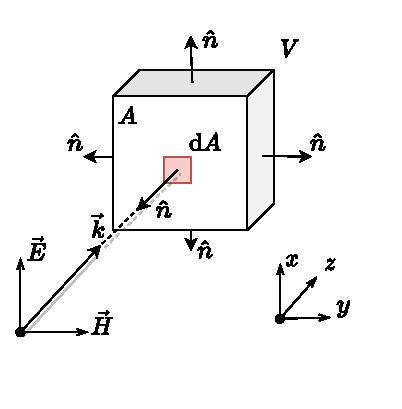
\includegraphics[width=0.46\textwidth]{artwork/exposed_tissue_volume.pdf}
    \caption{Exposed 10-g cubic volume for the assessment of the local exposure to \gls{em} fields.}
    \label{fig:exposed_tissue_volume}
\end{figure}
As this is not the case, it should be expected that $S_\text{ab, 1}$ will always yield values greater than $S_\text{ab, 2}$.
However, since above \SI{6}{\GHz}, power penetration depth is at most about \SI{8}{\mm}, this difference is marginal and thus may be disregarded as the overall contribution of absorption in deeper tissues is less then \SI{10}{\percent} at most.

\section{Incident Power Density}
The \gls{ipd} is used as the \gls{rl} in the \gls{icnirp} guidelines~\cite{ICNIRP2020Guidelines}, that is the \gls{erl} in the \gls{ieee} standard~\cite{IEEE2019Standard}.
It is defined as the modulus of the time-averaged Poynting vector,
\begin{align}
    \label{eqn:ipd}
    S_\text{inc} = |\mathbf{E} \times \mathbf{H}^* |.
\end{align}
In the case of the far-field exposure, it can be simplified to
\begin{align}
    \label{eqn:ipd-far-field}
    S_\text{inc} = \frac{|\mathbf{E}|^2}{Z_0} = |\mathbf{H}|^2 \; Z_0,
\end{align}
where $Z_0$ is the characteristic impedance of free space and it is about \SI{377}{\ohm}.
The above expression is a valid approximation whenever far-field conditions can be assumed which is generally during the assessment of either whole-body exposure or local exposure above \SI{6}{\GHz} if the antenna-to-tissue separation distance is above $\lambda / (2 \pi)$, where $\lambda$ is the wavelength of the incident field.
The said distance of $\lambda / (2 \pi)$ serves well to predict the margin between the reactive and radiative-near field~\cite{Carrasco2019Exposure}.
Because the plane wave reflection coefficient, $\Gamma$, can be used to correlate the incident and absorbed \gls{em} fields only under far-field conditions
\begin{align}
    \label{eqn:ipd-corr}
    S_\text{inc} = \frac{S_\text{ab}}{1 - |\Gamma|^2},
\end{align}
additional considerations are required for the near field.

In the far field, the Poynting vector is purely real, and the direction of the flux does not change in time.
In the near field of an antenna, this is no longer the case as reactive components of the field may contribute to the overall absorption of \gls{em} energy in the exposed body~\cite{Kuster1992Energy}.
Thus, all components of the Poynting vector should be considered to properly assess the \gls{ipd}, and the simple correlation-based formula as outlined in \cref{eqn:ipd-corr} is no longer accurate.

It is generally considered, and prescribed in both the \gls{icnirp} guidelines~\cite{ICNIRP2020Guidelines} and \gls{ieee} standard~\cite{IEEE2019Standard}, that the \gls{rl}/\gls{erl} cannot be used to determine compliance in the reactive near-field region and \gls{br}s/\gls{drl}s should be assessed instead.
However, in the recent \gls{ieee} Guide for the definition of the \gls{ipd} to correlate surface temperature rise~\cite{IEEE2021Guide}, two distinct definitions of the \gls{ipd} have been analyzed.

The first one is directly derived from the second definition of the \gls{apd} -- $S_\text{ab, 2}$ in this document, given in \cref{eqn:apd_2}, and it uses the normal components of the time-averaged Poynting vector in free space as follows
\begin{align}
    \label{eqn:ipd-normal}
    S_\text{inc, n} = \frac{1}{2A} \iint_A \Re \big( \mathbf{E} \times \mathbf{H}^* \big) \; \hat{\boldsymbol{n}} \; \mathrm{d}A,
\end{align}
where $\mathbf{E}$ and $\mathbf{H}$ are peak values of the complex phasor electric and magnetic field in free space, respectively.
The values of the \gls{em} field components are incident, rather than absorbed compared to the definition of the \gls{apd}.

The second definition considers all three components of the Poynting vector field (not solely the normal component) and thus takes into account the norm, i.e., the magnitude, of the power density vector.
It is written as follows
\begin{align}
    \label{eqn:ipd-magnitude}
    S_\text{inc, tot} = \frac{1}{2A} \iint_A \Big | \Re \big( \mathbf{E} \times \mathbf{H}^* \big) \Big | \; \mathrm{d}A.
\end{align}
Both equations for the assessment of the \gls{ipd} given in \cref{eqn:ipd-normal,eqn:ipd-magnitude} are concerning free space without any consideration of the interaction with the human body.
Because, in practice, the averaging area is often not a closed surface, the definition of the \gls{ipd} via the normal component of the Poynting vector may underestimate actual exposure.
Additionally, when the power density is assessed in the near-field region of a radiating source, where the tangential components of the Poynting vector are not negligible compared to its surface-normal components -- reactive-near field at distance $< \frac{\lambda}{2 \pi}$, the definition of the \gls{ipd} via its norm is shown to be slightly better correlated with maximum temperature rise.
However, this has been tested only considering several exposure scenarios in~\cite{IEEE2021Guide} and the overall analysis has shown that the observed difference is marginal and can mainly be attributed to near-field conditions as both definitions correlate well with temperature rise (correlation coefficients > 0.7).

% chapter 4
\clearpage
\chapter{The State of the Resarch}
\label{chap:results}

\section{Tissue Models}
The skin absorbs majority of incident \gls{rf} \gls{em} energy, and the power penetration depth is below about \SI{8}{\mm} and well below \SI{1}{\mm} at \SI{6}{\GHz} and \SI{30}{\GHz}, respectively.
Therefore, from the \gls{em} dosimetry point of view, tissue models should consist only of skin but a detailed knowledge of the internal skin structure is necessary to produce accurate predictions of \gls{rf} energy into tissue~\cite{Ziskin2018Tissue}.
On the other hand, from the thermal dosimetry point of view, it is necessary to include deeper tissues as well because the resulting surface temperature rise is determined by the thermal resistance of subcutaneous tissues even though the bulk of the \gls{em} energy is absorbed right at and slightly below the sole surface of the skin~\cite{Ziskin2018Tissue}.
As thermal modeling is out of the scope of this work, focus is put only on the tissue models for the \gls{em} dosimetry above \SI{6}{\GHz}. 

The details description of the structure of the skin, together with variations given age, sex and race, is outlined in~\cite{Snyder1979Report}.
The skin consists of two major layers -- the epidermis and dermis.
The epidermis is composed of five layers: the stratum corneum, stratum lucidum, stratum granulosum, stratum spinosum, and stratum basale.
Since the epidermis has no blood supply, but has a constant water content across all sub-layers (except stratum corneum which is water-free), it can be treated as the same layer when absorption of \gls{rf} energy is considered at and above \SI{6}{\GHz}.
The dermis consists of two layers: the papillary and reticular layer.
Additionally, the hypodermis, which is adipose tissue, lies beneath the dermis and has a much lower water content compared to the dermis.
Since fat has a low heat transfer coefficient, in this configuration, the overall upper skin layer acts as the thermal barrier.

Most of exposure assessment and/or computational dosimetry studies for local exposure above \SI{6}{\GHz} use planar tissue-equivalent single-, e.g.,~\cite{Nakae2020Skin,Poljak2020Assessment,Ziane2020Antenna}, or multi-layer models, e.g.,~\cite{Wu2015Safe,Foster2018Modeling,He2018RF}.
In the case of single-layer stratified models, typically the dielectric parameters of ``dry skin'' are considered and no detailed thermal anlysis is provided.
In the case of multi-layer models, either three or four distinct layers are considered as follows: the epidermis, dermis, hypodermis, and in some instances, muscle layer.
Dielectric properties are most often extracted by using the five-term Cole-Cole model~\cite{Gabriel1996Compilation}.  

\section{Spatial Averaging Considerations}
It is stated in the \gls{icnirp} guidelines~\cite{ICNIRP2020Guidelines} and the \gls{ieee} standard~\cite{IEEE2019Standard} that a square averaging area of \SI{4}{\cm\squared} provides a close approximation to maximum temperature rise due to \gls{rf} heating above \SI{6}{\GHz}.
This resolution is based mainly on thermal modeling study~\cite{Hashimoto2017On} where it is suggested that planar control surface for averaging with area of $2 \times 2$ \SI{}{\cm\squared}, shown in \cref{fig:averaging_surface}, is a good measure to correlate with the local peak temperature elevation when the field distribution is close to uniform within the area.
\begin{figure}[ht]
    \centering
    \begin{subfigure}[b]{0.51\textwidth}
        \centering
        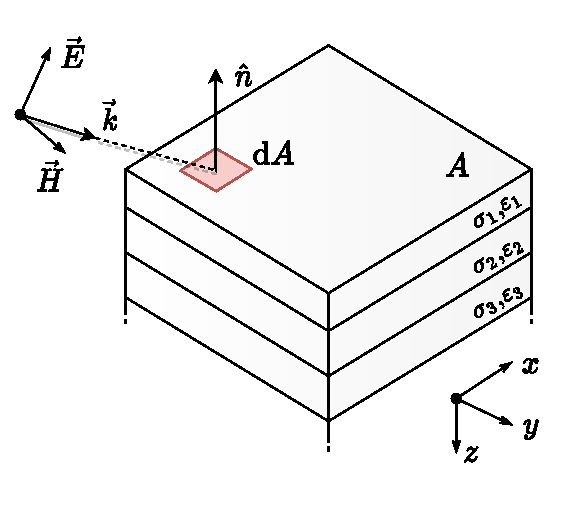
\includegraphics[width=\linewidth]{artwork/averaging_surface.a.pdf}
        \caption{3-D point of view.}
        \label{fig:averaging_surface_a}
    \end{subfigure}
    \begin{subfigure}[b]{0.42\textwidth}
        \centering
        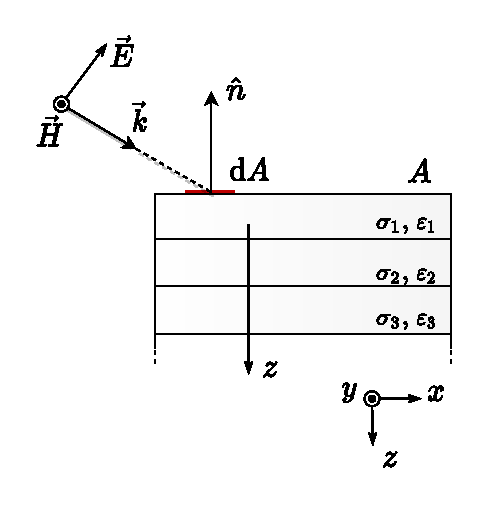
\includegraphics[width=\linewidth]{artwork/averaging_surface.b.pdf}
        \caption{Lateral point of view.}
        \label{fig:averaging_surface_b}
        \end{subfigure}
    
    \caption{Control surface for averaging on the multi-layer tissue-equivalent block model.}
    \label{fig:averaging_surface}
\end{figure}
The results from the study are based on the heating factor -- a ratio between the power density averaged on the area and maximum temperature rise on the same area, by considering a multi-layer tissue model exposed to three different sources of \gls{em} fields -- plane wave, a dipole antenna, and an antenna array.
The area of \SI{4}{\cm\squared} achieves consistency with the volume-averaged dosimetric quantities below \SI{6}{\GHz} as the front facing surface of 10-g cubic volume is about the same area ($2.15 \times 2.15$ \SI{}{\cm\squared} assuming constant tissue density of \SI{1000}{\kg\per\m\cubed}).

At higher frequencies (generally above \SI{30}{\GHz} for most exposure scenarios), the area of \SI{4}{\cm\squared} is not suitable because of the non-uniformity of the field distribution within such a large surface.
Thus, it is proposed in~\cite{Hashimoto2017On}, considering the results from the analytical study~\cite{Foster2016Thermal}, that the power density should be averaged on the most exposed area of \SI{1}{\cm\squared} for exposure above \SI{30}{\GHz} to better capture extremely focused beams.
An additional criterion is further imposed -- the (maximum) power density averaged over square \SI{1}{\cm\squared} area must not exceed 2 times the value for the corresponding averaging area of \SI{4}{\cm\squared}.

As the power density distribution, either incident or absorbed, on the front facing surface of the exposed tissue is computed numerically, it is of utmost importance to choose an appropriate averaging technique.
According to~\cite{Foster2022Three}, the \gls{fdtd} method was introduced to computational dosimetry and bioelectromagnetics in general in 1987 by Gandhi~\cite{Sullivan1987Use} as it was shown to be well adapted to \gls{em} computations at \gls{rf} frequencies.
Currently, the \gls{fdtd} method is the standard method in numerical dosimetry owing mostly to the advent of well-polished commercial software~\cite{Hirata2021Human}.
However, to achieve high-fidelity values of power density on the surface of conformal tissue-equivalent body models, especially at \gls{5g} frequencies, including \gls{mmw}, it is necessary to use methods that employ a structural instead of a grid-like spatial domain discretiztaion.
More details on this subject are available< elsewhere, e.g., in~\cite{Poljak2018On}.
In cases of regular grid, the surface is computationally reconstructed implicitly via cubical cells.
The spatial averaging is then crudely approximated as the averaged sum of contributions on each cell.
On the other hand, in cases of structural mesh, the surface is reconstructed by using the structural mesh composed of 2-D simplices for which there is a large array of corresponding efficient and accurate quadrature schemes, e.g., for disks~\cite{Kim1997Symemetric}, triangles~\cite{Dunavant1985High} and quadrilaterals~\cite{Dunavant1985Economical}.
The spatial averaging is then approximated by actually solving the surface integral of either the scalar (the first definition of the \gls{apd}, $S_\text{ab, 1}$, outlined in \cref{eqn:apd_1} and the norm definition of the \gls{ipd}, $S_\text{inc, tot}$, given in \cref{eqn:ipd-magnitude}) or vector field by using a 2-D quadrature technique of choice (the second definition of the \gls{apd}, $S_\text{ab, 2}$, outlined in \cref{eqn:apd_1} and the normal definition of the \gls{ipd}, $S_\text{inc, n}$, given in \cref{eqn:ipd-normal}).

\section{Local Exposure Assessment and Dosimetry Literature Review}
The current state of the literature is reviewed based upon the available studies accessible through the EMF-portal platform -- an internet information platform of the RWTH Aachen University which systematically summarizes scientific research data on the effects of \gls{em} fields on human body.
The core of the EMF-Portal is the literature database with 37,436 publications and 6,979 summaries of individual scientific studies\footnote{The total number of papers in the database was read on 2022, December 23rd at: \url{https://www.emf-portal.org/en}.}.

The following query was used to extract relevant studies:
\begin{verbatim}
    (power OR "power density")
    AND (average OR averaged OR area OR spatially)
    AND year=x
    AND (topic=technical_dosimetric
         OR topic=law_recommendation_guideline
         OR topic=review_survey_summary)
    AND (frequencyRange=radio_frequency
         OR frequencyRange=mobile_communications)
\end{verbatim}
where keywords are either ``power'' or ``power density'' together with either ``average'', ``averaged'', ``area'' or ``spatially''.
Keywords such as ``incident'', ``transmitted'', ``absorbed'' or even ``epithelial'' have been deliberately omitted in order to include both exposure assessment and computational dosimetry studies in the consideration regardless of authors' preference of terminology.
Additionally, the selected topics are technical dosimetry studies, laws, recommendation documents or guidleines associated with the aforementioned keywords, and review studies.
Finally, in the above query, the selected frequency range includes all bands that are classified within \gls{rf} and mobile communications ($f \geq \SI{10}{\MHz}$).
However, the purpose of this document is to review only the studies that pertain to spatial averaging of power density on the surface of the exposed tissue above \SI{6}{\GHz}.
Thus, additionally, only the studies which refer to the \SIrange[range-units=single,range-phrase=--]{6}{300}{\GHz} range are extracted manually.
This extraction was done per publication year of each research paper, from 1998 -- the year of publication of the previous version of the \gls{icnirp} guidelines~\cite{ICNIRP2020Guidelines}, ending with 2022 -- the year when this document was written.
A special emphasis is placed on the most recent studies, written after 2019 and 2020, when a new dosimetric quantity by means of the \gls{apd} was introduced in international exposure limits, and which is used for limiting local exposure to \gls{em} fields at the \SIrange[range-units=single,range-phrase=--]{6}{300}{\GHz} range.

\subsubsection*{1998 -- 2007}
During the 1998 to 2007 period, only a few of published studies addressed the spatial averaging of the power density on an exposed control surface, with only two studies considered exposure above \SI{6}{\GHz}.
This can be attributed to the fact that most wireless communication systems fell into the higher \SI{}{\MHz} range --  the \gls{em} power penetration depth is significant, thus \gls{sar} was considered a relevant dosimetric quantity.

However, limits to approximate exposure above \SI{10}{\GHz} in the far-field zone were given in terms of the \gls{ipd} spatially averaged on \SI{20}{\cm\squared} planar control surface in \gls{icnirp} 1998 guidelines~\cite{ICNIRP1998Guidlines}.
The \gls{ipd} was set to \SI{10}{\watt\per\meter\squared} and \SI{50}{\watt\per\meter\squared} for general public and occupational exposure, respectively.
Furthermore, local exposure was quantified by the spatially-averaged \gls{ipd} over the most exposed region of \SI{1}{\cm\squared} and was limited to \SI{200}{\watt\per\meter\squared} and \SI{1000}{\watt\per\meter\squared} for general public and occupational exposure, respectively.

In the \gls{ieee} standard published in 1999~\cite{IEEE1999Standard}, recommendations have been stated to prevent any potential adverse health effect by \gls{rf} \gls{em} fields and are intended to apply to exposures in both controlled (occupational exposure) and uncontrolled environments (general public).
Maximum permissible exposure is defined in terms of either the \gls{rms} electric and magnetic field strength, equivalent plane-wave power densities measured in free space, and currents induced within the human body to which a person may be exposed without adverse health effects and with an acceptable safety factor.
Above \SI{6}{\GHz}, the maximum permissible exposure in terms of the spatially-averaged power density for local body parts is set to a constant value of \SI{100}{\watt\per\meter} for occupational exposure, while it is defined as a function of frequency ($f / 150$) up to \SI{15}{\GHz}, but again set to a constant value of \SI{100}{\watt\per\meter} above \SI{15}{\GHz} for general public.
These values have been derived upon the \gls{br}s given by means of the stead-state volume-averaged \gls{sar}.
Spatial averaging is defined as the \gls{rms} of the power density over an area equivalent to the vertical cross section of the human body (projected area) at a distance of at least \SI{20}{\cm} from any object.

Given the maximum permissible exposure as defined in the previous two exposure limits~\cite{IEEE1999Standard,ICNIRP1998Guidlines}, in~\cite{Hirata2000Temperature}, the authors investigate temperature rise in the human eye for plane wave exposures at \SIrange[range-units=single,range-phrase=--]{0.6}{6}{\GHz}.
The numerical results are obtained by solving the Pennes bioheat equation~\cite{Pennes1948Analysis} with forcing term given by means of \gls{sar} given the specific frequency of impinging \gls{em} fields.
Maximum temperature rise due to the \gls{ipd} of \SI{50}{\watt\per\meter\squared} is \SI{0.3}{\celsius} at \SI{6}{\GHz}.
The value of the \gls{ipd} is chosen to match the maximum permissible exposure limit for occupational exposure as per~\cite{Ulcek1997Evaluating}.
In this document, spatial averaging is performed by taking the mean value of the power density over an area approximately equivalent to the vertical cross-section (projected area) of the exposed part of the human body.

In human study~\cite{Walters2000Heating}, thermal pain thresholds were measured in 10 subjects during brief exposure at \SI{94}{\GHz} with the \gls{ipd} set to extremely high value of \SI{18}{\kW\per\meter\squared}.
It is found that the pain threshold for pricking pain is \SI{43.9}{} $\pm$ \SI{0.7}{\celsius} (\SI{95}{\percent} confidence interval, which corresponds to the maximum surface temperature rise of about \SI{9.9}{\celsius}.
The results are in a very good agreement with the simple 1-D analytical model based on the Pennes bioheat equation~\cite{Pennes1948Analysis}.
In this study, the \gls{ipd} is spatially averaged over the planar projection of the human back in 2-D.
For purposes of specifying the \gls{ipd}, the spatial averaging is performed simply by computing the mean power density within the most exposed region (where \SI{90}{\percent} of the total incident power density was distributed).

Finally, in~\cite{Faraone2000Estimation}, a set of analytical formulas has been postulated to estimate the averaged power density in the close proximity of base-station collinear array antennas.
Authors suggest that the \gls{ipd} averaged over the whole body can be used to verify compliance to maximum permissible exposure limits for antenna-to-body separation distances larger than $\lambda/2$ where there is no significant coupling between the antenna and body and where electrical properties of the antenna are constant during exposure.
Further, under the assumption of the cylindrical character of \gls{em} fields in the immediate vicinity of the array, the average power density is given as:
\begin{align}
    \bar{P}_\text{d}(\rho) \approx \frac{P_\text{rad}}{2L \cdot 2\pi\rho},
\end{align}
where
\begin{align}
    P_\text{rad} \approx 2\pi\rho \int_{-L}^{L} \Re \Big( \frac{1}{2} \; E_z \; H_\Phi^* \Big),
\end{align}
and where $P_\text{rad}$ represents the power radiated by the collinear array of half-wavelength dipole antennas with $2N +1$ radiating elements, each excited by a time-harmonic current, $I_n$.
Other parameters are as follows: $2L$ is the overall length of the antenna with each element separated from each other by the distance $p \leq \lambda$, $\rho$ is the distance away from the antenna, $E_z$ and $H_\Phi$ are the amplitude of the $z$-component of the electric and the $\Phi$-component of the magnetic field, respectively.
With an increase in distance from the antenna, the above quantity undergoes transition from the cylindrical decay in the near field, to the spherical in the far field (details available in subsection B of section II in~\cite{Faraone2000Estimation}).
The main contribution of this paper is the outlined set of formulas for the accurate prediction of the average exposure from different sources, from collinear arrays to other directive antennas.
These formulas can be adjusted to take into account the partial exposure as:
\begin{align}
    \bar{P}_\text{d}(\rho, L; T, H) \approx P_\text{d}(\rho, L) \cdot \frac{T}{H}, \quad \rho << G_A \; L,
\end{align}
where $G_A$ stands for the collinear array broadside gain, and where $T$ and $H$ represent the height of the person standing parallel in front of the antenna and $t$ is the intercepted portion.
The advantage of using the concept of average power density as presented in this work is the simplicity of evaluation of the exposure of humans near cellular base-station antennas, but unfortunately it does not take into account an actual local exposure and predicts only a single-point measure of the worst-case \gls{ipd}.

In the revised version of the \gls{ieee} 1999 standard~\cite{IEEE1999Standard}, it was prescribed that the exposure limit for general public given by means of the spatially-averaged \gls{ipd} is \SI{10}{\W\per\m\squared} at \SIrange[range-units=single,range-phrase=--]{3}{10}{\GHz} range.
The power density should be spatially averaged over any contiguous area corresponding to $100 \lambda^2$.
In addition, maximum spatial peak power densities of $18.56 \cdot f_G^{0.699}$
and \SI{200}{\watt\per\m\squared} were defined at the \SIrange[range-units=single,range-phrase=--]{3}{30}{\GHz} 
and above \SI{30}{\GHz}, respectively, where $f_G$ is the frequency of the impinging \gls{em} field in \SI{}{\GHz}.
However, no averaging area or spatial sampling density was officially specified to assess the spatial peak power density limits.

\subsubsection*{2008 -- 2017}
In two studies published by the same research group, the question of what is the appropriate exposure metric at the \SIrange[range-units=single,range-phrase=--]{1}{10}{\GHz} range -- \gls{sar} or \gls{ipd}, is discussed by using the simple 1-D planar model~\cite{Anderson2010SAR} and complex human body models~\cite{McIntosh2010SAR}.

In the first study~\cite{Anderson2010SAR}, the most appropriate transition frequency at which the \gls{ipd} should replace volume-averaged \gls{sar} as the \gls{br} is discussed.
It is based on Monte Carlo analysis with varying input parameters such as tissue thicknesses and body sites.
The results show that the peak \gls{sar} is better indicator of maximum surface temperature rise across the entire examined spectrum compared to the \gls{ipd}.
Furthermore, peak 10-g \gls{sar} achieves only marginally better predictive power than its 1-g counterpart.
As the tissue is represented by using the 1-D multi-layer model, no spatial averaging is conducted to evaluate the \gls{ipd}, which is addressed in the subsequent study~\cite{McIntosh2010SAR}.

Instead of 1-D planar tissue models, in~\cite{McIntosh2010SAR}, complex human body models, i.e., heterogeneous head models of an adult and a 12-year-old, for a variety of exposure scenarios have been utilized to assess the frequency at which the transition in \gls{br} -- from \gls{sar} to \gls{ipd}, is appropriate.
Numerical results show that the maximum temperature rise on the surface correlate better with the peak 10-g \gls{sar} up to \SI{6}{\GHz} compared to the \gls{ipd}.
On the contrary to the previous analytical study~\cite{Anderson2010SAR}, above \SI{6}{\GHz}, the results show significantly better correlation of the \gls{ipd} with maximum temperature rise.
Considering combined conclusions from both studies, authors suggest that the transition frequency should be set to \SI{6}{\GHz}.

Discussion on the transition frequency is conducted in~\cite{Colombi2015} where the implication of this transition is further addressed by means of the the maximum possible radiated power from a device used in close proximity to the human body.
The results of this study have demonstrated the non-physical discontinuity in the maximum radiated power as the transition is made from \gls{sar} to the \gls{ipd}.
This means that devices should use significantly lower radiated power (in order of several \SI{}{\decibel}) to achieve compliance above \SI{6}{\GHz}.
Two key observations of this study are as follows: (i) the necessity of the harmonization of the transition frequency for \gls{br}s across all internationally defined exposure limits by standardization organizations and regulatory authorities, and (ii) averaging areas in~\cite{ICNIRP1998Guidlines,IEEE2005Standard} are not appropriate and lead to inconsistency in defining exposure above the transition frequency.

Similar conclusions have been outlined in~\cite{Thors2016Exposure} where complex numerical simulations of exposure to array antennas in \gls{5g} mobile communication equipment have been conducted.
Here, a systematic study varying parameters such as the frequency, array size, array topology, antenna-to-body separation distance, and beam steering range is considered and compared to the measured data.
Overall conclusion is that a global harmonization of the exposure limits above \SI{6}{\GHz} is necessary to avoid unjustified decrease of the maximum transmitted power of \gls{5g} user equipment compared to preceding generations.
The spatial averaging of the power density in this paper is conducted as defined in \cref{eqn:ipd-normal}.

Furthermore, as a sequel to results presented in~\cite{Colombi2015,Thors2016Exposure}, in~\cite{Xu2017Understanding}, the difference between definitions of the maximum spatially-averaged power density and the influence of different interpretations on the maximum permissible transmitted power of user equipment mock-ups employing a patch array operating at \SI{15}{\GHz} have beem presented.
First interpretation is taken from~\cite{Thors2016Exposure} where \gls{ipd} is spatially averaged on the square shaped control surface by following the formulation given in \cref{eqn:ipd-normal}.
Surface integral of the vector field is approximated to obtain the total power flux density that passes through the averaging area and subsequently normalized with that area.
The second interpretation is the maximum arithmetic mean value of the power density over the averaging area, analogous to \cref{eqn:ipd-magnitude}.
The main difference is that in the first interpretation only the normal components of the power density vector are considered, whereas in the second definition tangential components are included.
In the reactive near-field zone, there is always an antenna-body coupling present due to the reflected \gls{em} power density flowing back inwards user equipment, it is thus reasonable to expect that the second interpretation will yield results that are greater than the values obtained by the first interpretation of the spatially-averaged \gls{ipd}.
Numerical results demonstrate the overall dependence of the difference of maximum permissible transmitted power to comply with the \gls{icnirp} 1998 guidelines~\cite{ICNIRP1998Guidlines} are \SIrange[range-units=single,range-phrase=--]{1}{2.6}{\decibel} depending on the antenna-to-body separation distance.
Authors here again appeal that all regulatory organizations should not only agree upon the transition frequency but also to explicitly state the definition of the maximum spatially-averaged \gls{ipd} to remove any exiting ambiguities.

Finally, the research outlined so far culminates in the publication of the seminal work~\cite{Hashimoto2017On} where the authors discuss both the averaging area for the \gls{ipd} and the transition frequency.
The relationship between the size of the area over which incident power density is averaged and the local peak temperature elevation in a tissue-equivalent multi-layer model by means of the heating factor has been reported.
This relationship is based on the numerical data obtained by simulating exposure of the model to different radiating sources (plane-wave, half-wavelength dipole, and dipole array) at the \SIrange[range-units=single,range-phrase=--]{3}{300}{\GHz} range.
It has been shown that over \SI{70}{\percent} of the absorbed power is located within the boundaries of the \SI{4}{\cm\squared} region on the most exposed surface which mostly determines maximum surface temperature increase.
Thus, an averaging area of $2 \times 2$ \SI{}{\cm\squared} provides a good measure to correlate with local peak temperature rise when the field distribution is nearly uniform across that area.
Additionally, above \SI{30}{\GHz}, the averaging should be performed on $1 \times 1$ \SI{}{\cm\squared} averaging surface to account for localized beam formation and to capture non-uniformities.
These findings have served exceptionally well for defining the revised version of the \gls{ieee} standard and \gls{icnirp} guidelines that followed in 2019 and 2020, respectively.

\subsubsection*{2018-present}
In~\cite{Christ2018Thermal}, the analysis of temperature rise on the surface of single- and multi-layer- tissue-equivalent models positioned in close proximity to generic \gls{5g} wireless devices with phased array antennas operating at \SI{28}{} and \SI{100}{\GHz} has been presented.
Temperature increase is quantified in relation to both the electric field amplitude to take into account the possible impact of reactive components of the incident field in the near-field zone, and the real part of the power density flux across \SI{20}{} and \SI{1}{\cm\squared} planar control area on the exposed surface of the model.
Authors argue that the size of the averaging area along with the layering structure of the tissue are two most important parameters for exposure assessment and temperature increase on the surface.
For an averaging area of \SI{1}{\cm\squared}, normalization of surface temperature rise to both the electric field and \gls{ipd} yield similar results, whereas an averaging area of \SI{20}{\cm\squared} shows differences depending on the normalization for the smaller antenna array at \SI{100}{\GHz}.
The overall conclusion is that the spatially-averaged\gls{ipd} represents an accurate proxy for temperature rise and can serve to assess compliance provided the averaging surface is appropriately defined with regard to the exposure scenario.
Finally, authors call for the urgent need of additional analysis to establish a robust correlation of the averaged power density values with the induced temperature increase as well as to establish the most suitable shape of the surface for averaging.

In line with~\cite{Hashimoto2017On}, in~\cite{Funahashi2018Averaging}, additional analysis of the \gls{ipd} spatially-averaged on the square surface of \SI{1}{} and \SI{4}{\cm\squared} at the \SIrange[range-units=single,range-phrase=--]{10}{100}{\GHz} range has been performed.
The correlation with maximum temperature rise on the exposed surface is examined for the case of patch antenna arrays with 4 by 1, 2 by 2, and 3 by 3 elements, and compared with 1-D analysis~\cite{Foster2017Thermal}.
It is confirmed that the \SI{4}{\cm\squared} averaging area is suitable up to \SI{30}{\GHz}, but the smaller averaging area is needed above \SI{30}{\GHz} because the non-uniform \gls{em} field distribution.
Additionally, this study finds that the square shaped averaging area of \SI{4}{\cm\squared}, characterized by the heat diffusion length, should be the most appropriate by means of the shape and size considering it corresponds to the face area of the \gls{sar} averaging 10-g volume under the assumption that the mass density is \SI{1000}{\kg\per\meter\cubed}~\cite{Hirata2019Setting}.
This leads to preserved consistency in the ratio of maximum temperature rise in the skin to the \gls{sar} averaged over \SI{10}{\g} of tissue, which is confirmed to be a valid metric to assess compliance~\cite{Hirata2003Temperature,Hirata2009correlation,McIntosh2010SAR}.

Authors of the same group as in~\cite{Funahashi2018Averaging} performed computations of the area-averaged \gls{tpd} at the skin as a new potential metric to estimate the steady-state skin temperature elevation above the transition frequency.
The results were obtained at \SIrange[range-units=single,range-phrase=--]{3}{300}{\GHz} for the case of multi-layer homogeneous cube with dielectric and thermal properties of the skin and additionally compared to the realistic human body model.
Numerical results have shown excellent agreement with 1-D analytical solution first presented in~\cite{Foster2017Thermal} and confirm the area-averaged \gls{tpd} as a potential surrogate of surface temperature rise.
The averaging area of \SI{4}{\cm\squared} again have been shown as appropriate for frequencies up to \SI{300}{\GHz} provided that they are supplemented by limits on the intensity of very small beams.
If not, the reduction of an averaging area by a factor of 4 for small beamwidths should be a reasonable choice, and provides continuity with far-infrared guidelines $ > \SI{300}{\GHz}$.
A large contribution of this study is the introduction of a new metric of the power density that is no longer measured in free space but rather represents the internal/dosimetric quantity for estimating surface temperature above transition frequency.
During the time of writing~\cite{Funahashi2018Averaging}, this metric was discussed and mentioned in the \gls{icnirp} public consultation document and \gls{ieee} C95.1 draft for the 2019 version of the \gls{ieee} standard~\cite{IEEE2019Standard}.
Mathematically, it is identical to \cref{eqn:tpd} and, once averaged, should correspond to \cref{eqn:apd_1} which is currently the official \gls{br} above \SI{6}{\GHz} in both the \gls{ieee} C95.1-2019 standard~\cite{IEEE2019Standard} and \gls{icnirp} 2020 guidelines~\cite{ICNIRP2020Guidelines} for limiting local steady-state exposure.
Unfortunately, the spatial averaging in this work is not explicitly outlined.
It is stated, however, that the spatially-averaged \gls{tpd} is approximated by multiplying a transmission coefficient by the \gls{ipd}, which is obtained beforehand as the magnitude of the Poynting vector in free space averaged over an area of either \SI{4}{} or \SI{1}{\cm\squared} (in square shape), depending on frequency, on the plane where the model surface exists.

Two studies~\cite{He2018RF,Miura2021Power} have performed \gls{rf} compliance analysis of surface temperature elevation in human head model at \SI{28}{\GHz} realistic sources, e.g., beam-steering patch arrays, dipoles, etc., which was the expected frequency for the \gls{5g} commercial products.
In~\cite{He2018RF}, authors confirm that the power density averaged over \SI{1}{\cm\squared} in free space, i.e., the spatially-averaged \gls{ipd}, and the maximum surface temperature rise have good correlation, which is further verified by performing 1-D analysis concerning plane-wave exposure. 
In this study, authors discuss both definitions, i.e., the norm and normal definition, of the \gls{ipd} as given in \cref{eqn:ipd-magnitude,eqn:ipd-normal}, respectively, but adopt the norm definition as it results in higher power density values by taking into account tangential components of the incident field, and thus represents potentially more conservative value to treat the maximum permissible transmitted power.
In a latter study~\cite{Miura2021Power}, authors investigate simultaneous near-field exposure at \SI{2}{\GHz} in addition to \SI{28}{\GHz} from the inverted-F and patch array antenna, respectively.
At \SI{2}{\GHz}, 10-g volume-averaged \gls{sar} is used a surrogate for temperature rise, whereas at \SI{28}{\GHz}, the spatially-averaged \gls{tpd}, i.e., the first definition of the \gls{apd} as presented in this document in \cref{eqn:apd_1}, is used.
Overall, computational results showed that the effect of superposition is marginal and can be attributable to the heat diffusion length in biological tissues.
Outlier is found for the case when patch antenna array and inverted-F antenna were separated by less than \SI{50}{\mm} at the \SI{5}{\mm} antenna-to-tissue separation distance where the effect of the superposition was \SI{15}{\percent} greater.

The averaged area for \gls{ipd} calculation is analyzed, and dependence on the incident angle and frequency is studied in~\cite{Poljak2018On}.
The authors adopt the normal definition of the \gls{ipd} as presented in \cref{eqn:ipd-normal} but adjusted into the analytical expression that pertains to field components of the half-wavelength dipole antenna operating in free space at multiple frequencies within the \SIrange[range-units=single,range-phrase=--]{3}{300}{\GHz} range.
It has been shown that the derived analytical expression is convenient for a rapid estimation of the \gls{ipd} in the equatorial plane of the half-wavelength dipole which simultaneously represents a worst case scenario of local exposure.

More complex numerical analysis regarding the effect of incidence angle on the spatially-averaged \gls{ipd} to correlate skin temperature rise at \SI{30}{\GHz} rise for has been provided in the intercomparisson study~\cite{Diao2021Effect}.
Both definitions of \gls{ipd} spatially-averaged across \SI{1}{\cm\squared} have been compared for the exposure of a multi-layer tissue-equivalent block model to 4 by 4 array antenna.
The influence of multiple input parameters such as the antenna type, antenna-to-tissue separation distance, and overall skin model to the computed \gls{ipd} have been discussed based on the results that have shown both definitions are in good agreement and correlate well with maximum temperature rise for small or moderate incidence angles.
The normal definition of \gls{ipd} is shown to be less dependent of the incidence angle than the norm definition which tends to decrease rather significantly for large incidence angles.
For exposure to the transverse-magnetic polarized incident waves at the Brewster angle, heating factor regarding the norm definition is enhanced -- the normal definition is less conservative than the norm definition.
This effect is observed for large antenna-to-tissue separation distances.
Overall, normal incidence has been shown to be the worst case scenario generally across different exposure scenarios and should be considered during compliance assessment, which is in line with the conclusion of the aforementioned analytical study~\cite{Poljak2018On}.

Until now, it is clear that for the spatially-averaged power density and associated surface temperature rise are functions of the angle of incident wave to that surface~\cite{Hirata2021Assessment}.
It has been shown in~\cite{Li2019Relationship} that the transmittance of the transverse-magnetic incident wave increases with the increasing angle up to the maximum transmittance angle owing to the Brewster effect.
This study performed Monte Carlo analysis to derive to this conclusion where, again in line with studies~\cite{Poljak2018On,Diao2021Effect}, it has been shown that the normal incidence corresponds to the worst case local exposure scenario.
Additionally, the results demonstrate that at the \SIrange[range-units=single,range-phrase=--]{6}{1000}{\GHz} range, \gls{tpd} strongly correlates with surface temperature rise and provides a suitable quantity for evaluating \gls{em} dosimetry above \SI{6}{\GHz}.

In~\cite{Li2021Quantitative}, a quantitative comparison of both the spatially-averaged \gls{ipd} and \gls{apd} related to near-field exposure at \SIrange[range-units=single,range-phrase=--]{6}{100}{\GHz} has been provided.
This study took both definitions of the \gls{ipd} -- the spatially-averaged magnitude of the complex Poynting vector \cref{eqn:ipd-magnitude} and spatially-averaged norm of the real part of the complex Poynting vector \cref{eqn:ipd-magnitude}, and assess their relationship with the \gls{apd} and correlation with maximum surface temperature rise.
The analysis pertains to the normally incident \gls{em} waves radiated by the single half-wavelength dipole, 1 by 4 and 4 by 1 dipole array antennas onto the multi-layer planar tissue-equivalent model at the separation distance in the range of \SIrange[range-units=single,range-phrase=--]{2}{10}{\mm}.
Out of the reactive near-field zone (approximately at the distance $> \lambda / (2 \pi)$), there exists only a marginal difference between the two definitions of the \gls{ipd} (within \SI{0.7}{\decibel}).
Difference between the norm and normal definition of the \gls{ipd} compared to the spatially-averaged \gls{apd} are \SI{0.9}{} and W\SI{1.4}{\decibel}, respectively.
Within the near reactive near-field zone, \gls{ipd} is not appropriate metric do assess compliance and thus is not considered in such cases.
Overall, the results suggest that the definition of the \gls{ipd} be that the norm or normal definition is not significant factor that influences exposure assessment unlike other factors such as the frequency, antenna-to-tissue separation distance, and the size of the averaging area.
Similar conclusions have been derived in~\cite{DeSantis2022On}.
Additionally, these conclusions have been verified in the intercomparisson study~\cite{Li2021Intercomparison}.
This study clarifies the main causes of numerical errors in dosimetry analysis by having computation results from six different organizations worldwide compared using their own separate numerical methods with different various body and antenna models.
Details are omitted for the sake of brevity but, in  general, the fair agreement among research groups have shown that numerical calculation errors of dosimetry analysis caused by the definition of spatially averaged incident power density are marginal.

Recently, the \gls{ieee} guide for the definition of the \gls{ipd} to correlate maximum surface temperature rise has been published~\cite{IEEE2021Guide} where the main goal is to clarify all ambiguities related to the mathematical definition of the \gls{ipd}, averaging surface, usage, incident angle and other confounding variables.
This guide includes different exposure scenarios -- exposure from different radiating source, incident angles and frequencies within the \SIrange[range-units=single,range-phrase=--]{10}{90}{\GHz} range at separation distances of \SIrange[range-units=single,range-phrase=--]{2}{150}{\mm}.
In addition to statistical analysis, results have been verified with thermographic measurements.
Three important general conclusions have been derived upon the presented results: (i) the norm definition of the \gls{ipd} results in highest correlation coefficients with temperature, however, both definitions correlate strongly with temperature rise for the scenario of quasi-perpendicular incidence (Pearson correlation coefficients $> 0.7$), (ii) the norm definition yields a better estimate of the induced temperature increase than the normal definition but this difference is marginal and is present only when the near-field conditions are considered, and (iii) the heating factor as a function of the angle of incidence shows that the normal definition of the \gls{ipd} correlates better with maximum surface temperature rise compared to the norm definitions as it is less sensitive to the incidence angle variation, but the use of the norm definition results in more conservative exposure estimates.

It is also important to note that in~\cite{Christ2020Limitations}, an additional definition of the \gls{ipd} has been considered for local exposure assessment at multiple separation distances from different simplistic and realistic antennas, e.g, the dipole, loop, slot, patch, and helix antenna.
Namely, to be able to evaluate the impact of the reactive near-field during exposure assessment, it is important to considered imaginary components of the Poynting vector as well.
Thus, the third proposed definition is given as:
\begin{align}
    S_\text{inc, im} = \frac{1}{2A} \iint_A \big| \mathbf{E} \times \mathbf{H}^* \big| \; \mathrm{d}A.
\end{align}
Given the presented results, authors have concluded that above definition yields a better proxy for the \gls{apd} in the near-field zone in comparison to two standard definitions as it takes into account losses that are induced by the reactive field components which cannot be found in the real part of the Poynting vector.
In addition to proposed surface areas of \SI{4}{} and \SI{1}{\cm\squared}, the analysis also includes frequency-dependent surface area of $(\lambda / 4)^2$.
By spatially averaging the power density across this frequency-dependent surface, it is possible to avoid underestimation of the \gls{apd} that otherwise could happen in cases when using fixed normalizing surface areas.
Since the authors based these conclusion without taking into consideration the relationship with maximum surface temperature rise whereas the exposure safety limits pertain first and foremost to the issue of tissue heating, this definition has not been considered in most of the subsequent literature.

\subsubsection*{Future Directions}
A working group 5 under Subcommittee 6 of \gls{ieee} International Committee on Electromagnetic Safety Technical Committee 95 has established two distinct definitions of the \gls{ipd} spatially averaged over an evaluation plane -- a control surface on the irradiated planar projection of human skin in free space, of area \SI{4}{} or \SI{1}{\cm\squared} depending on the operating frequency in~\cite{IEEE2021Guide}.
To date, most of exposure assessment and \gls{em} dosimetry studies above \SI{6}{\GHz}, including \gls{mmw}, use planar tissue-equivalent single-~\cite{Nakae2020Skin,Poljak2018On,Poljak2020Assessment,Ziane2020Antenna,Kapetanovic2021Application} or multi-layer~\cite{Wu2015Safe,Wu2015human,Foster2018Thermal,Ziskin2018Tissue,He2018RF,Carrasco2019Exposure,Diao2021Effect,Li2021Quantitative} models.
However, one issue in such approach is the assessment of power densities on non-planar body parts with the curvature radius on the same scale as the wavelength of the incident \gls{em} field~\cite{Sacco2022Exposure,Kapetanovic2022Assessment,Kapetanovic2022AssessmentJERM}.
This has been already addressed at the \SIrange[range-units=single,range-phrase=--]{900}{3700}{\MHz} range considering the absorption of electromagnetic fields in human hands~\cite{Li2012Mechanisms}.
The results comparing the absorption in the hand versus a standardized flat phantom have shown enhancements of several \SI{}{\decibel}, which is most likely due to the fingers having their own resonance modalities for the absorption of \gls{rf} \gls{em} energy at such frequencies.
Furthermore, the influence of the curvature of different body parts modeled by using canonical geometries, e.g., cylinder or elongated cylinder, with radii of the order of several \SI{}{\mm} at \gls{mmw} have been investigated in~\cite{Sacco2022Exposure}, but due to the reduced model dimensions, no spatial averaging has been considered.

Currently, a working group 7 under Subcommittee 6 of \gls{ieee} International Committee on Electromagnetic Safety Technical Committee 95 has been establish with the aim of defining new averaging schemes for the assessment of the \gls{apd}.
Other than common evaluation plane, two different surfaces have been proposed: a spherical and cylindrical surface.
Examples of the spherical and cylindrical model with radius set to \SI{5}{\cm} are shown in \cref{fig:cylinder,fig:sphere}, respectively.
In \cref{fig:cylindrical_surface,fig:spherical_surface}, the positional relationship of non-planar averaging surfaces with the control evaluation plane is shown.
\begin{figure}[ht]
    \centering
    \begin{subfigure}[b]{0.42\textwidth}
        \centering
        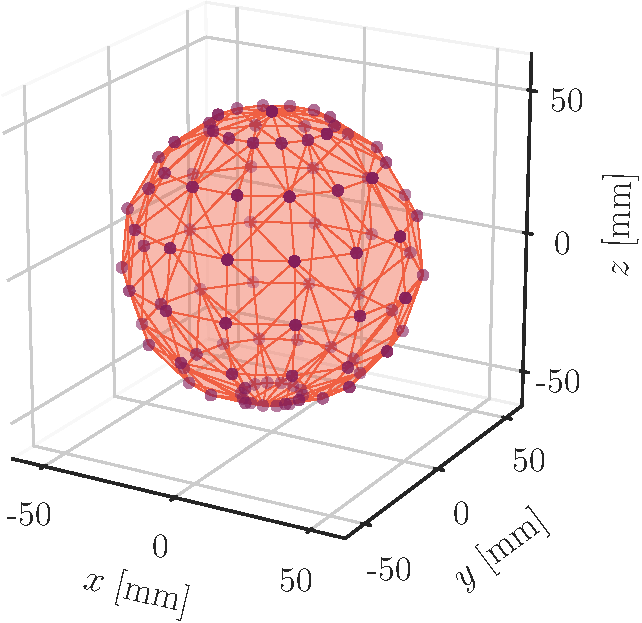
\includegraphics[width=\linewidth]{artwork/spherical_model.pdf}
        \caption{Spherical model.}
        \label{fig:spherical_model}
    \end{subfigure}
    \hfil
    \begin{subfigure}[b]{0.47\textwidth}
        \centering
        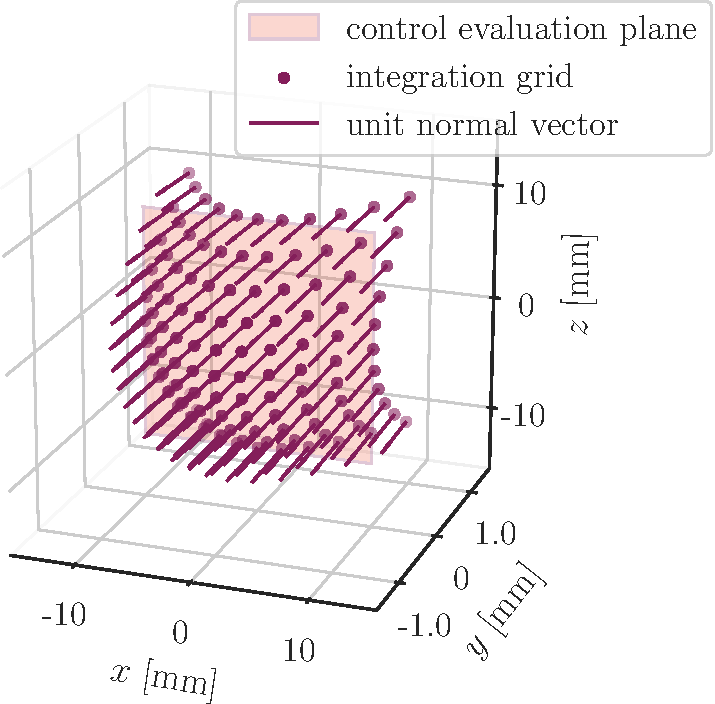
\includegraphics[width=\linewidth]{artwork/spherical_surface.pdf}
        \caption{Spherical averaging surface.}
        \label{fig:spherical_surface}
        \end{subfigure}
    
    \caption{Spherical model with radius set to \SI{5}{\cm}. Spherical averaging surface of \SI{4}{\cm\squared} is represented with integration points that serve as an origin to unit vector field distributed across that surface.}
    \label{fig:sphere}
\end{figure}
\begin{figure}[ht]
    \centering
    \begin{subfigure}[b]{0.42\textwidth}
        \centering
        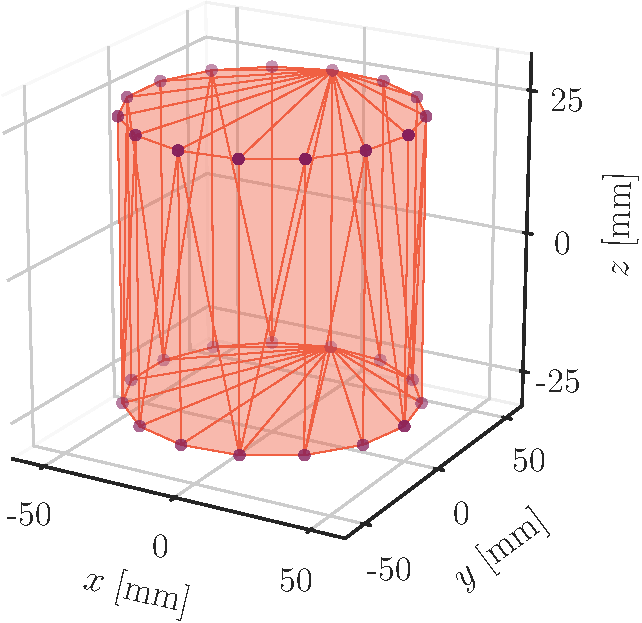
\includegraphics[width=\linewidth]{artwork/cylindrical_model.pdf}
        \caption{Cylindrical model.}
        \label{fig:cylindrical_model}
    \end{subfigure}
    \hfil
    \begin{subfigure}[b]{0.47\textwidth}
        \centering
        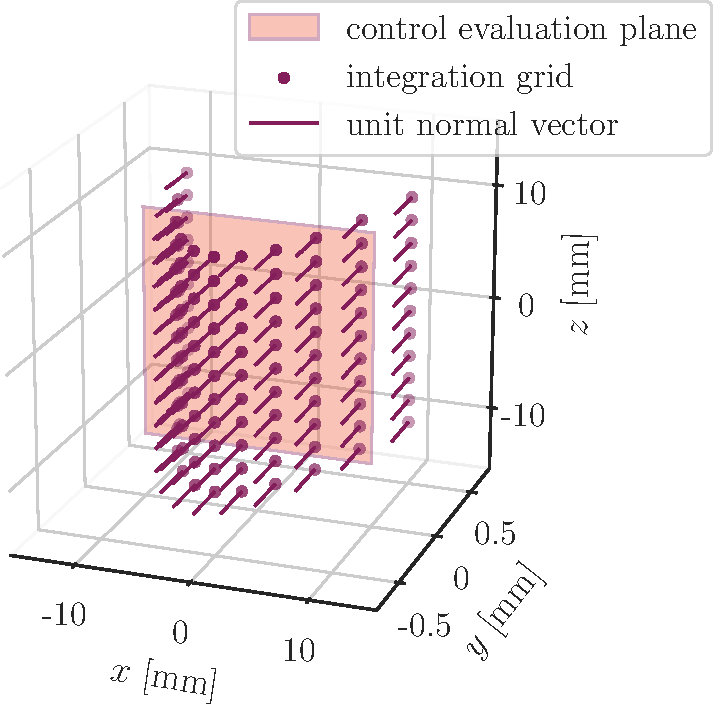
\includegraphics[width=\linewidth]{artwork/cylindrical_surface.pdf}
        \caption{Cylindrical averaging surface.}
        \label{fig:cylindrical_surface}
        \end{subfigure}
    
    \caption{Cylindrical model with radius and height both set to \SI{5}{\cm}. Cylindrical averaging surface of \SI{4}{\cm\squared} is represented with integration points that serve as an origin to unit vector field distributed across that surface.}
    \label{fig:cylinder}
\end{figure}

Some of the proposed averaging techniques, which are currently being discussed within a working group 7 under Subcommittee 6 of \gls{ieee} International Committee on Electromagnetic Safety Technical Committee 95, are directly motivated by the schemes proposed in~\cite{Diao2020Assessment}.
In this work, the assessment of the \gls{apd} on non-planar canonical surfaces at the \SIrange[range-units=single,range-phrase=--]{6}{60}{\GHz} range for a realistic forearm model~\cite{Diao2020Assessment} have been proposed.
Given the body parts are represented as the voxelized models, authors have adopted the definition of the \gls{apd} as given in \cref{eqn:apd_1} for practical reasons and for ease of computation.
Four distinct schemes for the spatial averaging of the \gls{apd} have been presented and are shown in \cref{fig:diao2020assessment}.
The definition of the integration volumes for different schemes are bounded by red polygons as follows.
The upper bound, L1, is parallel to the grid axis in \cref{fig:diao2020assessment}(a) and \cref{fig:diao2020assessment}(b) to match the standard evaluation plane commonly encountered in literature.
On the other hand, the upper bound, L1, is bent along the surface to approximately match the curvature of skin in \cref{fig:diao2020assessment}(c) and \cref{fig:diao2020assessment}(d).
Side bounds, L2 and L3, are parallel to the grid axis in \cref{fig:diao2020assessment}(a) and \cref{fig:diao2020assessment}(c),  whereas in \cref{fig:diao2020assessment}(b) and \cref{fig:diao2020assessment}(d), L2 and L3 are parallel to the internal electric field gradients at the model surface.
In all schemes, the lower bound, L4, is defined as the contour where the electric field is at $1/1000$ of the maximum value in the integration volume.
\begin{figure}[ht]
    \centering
    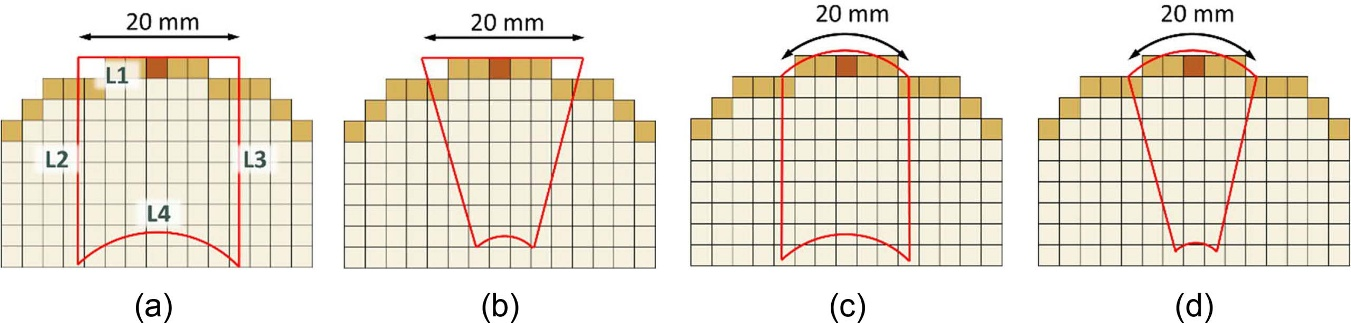
\includegraphics[width=\textwidth]{artwork/Diao2020Assessment_figure2.png}
    \caption{Figure 2. in~\cite{Diao2020Assessment}: ``Definitions of the integration volumes for the different absorbed power density calculation schemes. (a) Scheme 1, (b) Scheme 2, (c) Scheme 3, and (d) Scheme 4.''}
    \label{fig:diao2020assessment}
\end{figure}
As these types of voxelized representations of the human body are known to suffer from stair-casing numerical errors~\cite{Poljak2018On}, a novel local compensation method has been established which allows for correcting the heat convection rate and is validated by the analytical solution by using a simple spherical model and prolate ellipsoidal models. 
Overall, authors conclude that for the model curvature radius $> \SI{30}{\mm}$ at and above \SI{20}{\GHz}, the heating factors agree well with those obtained in previous studies using planar models, and the differences in the heating factors among different proposed schemes for assessment of the spatially-averaged \gls{apd} on non-planar surfaces are marginal.

\Gls{em} exposure assessment of the \gls{ipd} on spherical head model up to \SI{100}{\GHz} is provided in~\cite{Kapetanovic2022AssessmentTEMC}.
In this study, the radiating source was modelled as the half-wavelength dipole antenna placed in close proximity of the spherical model with radius corresponding to that of the average human male.
It has been shown that the spatial averaging of the incident power density at the \SIrange[range-units=single,range-phrase=--]{3.5}{100}{\GHz} range yields to up to \SI{30}{\percent} greater values compared to the common planar surface.
Interestingly, authors positioned the evaluation plane at three distinct locations with respect to the spherical averaging surface which closely resembles the one shown in \cref{fig:spherical_surface}.
Namely, the first planar averaging surface corresponding to the worst case exposure scenario is placed onto a tangential plane of the nearest point on the spherical averaging surface.
The second planar averaging surface is located on a plane intersecting the spherical averaging surface at 4 points in the middle – between the nearest point and 4 farthest points on the surface of the spherical averaging surface relative to the antenna position.
Finally, the last considered planar averaging surface intersects the spherical averaging surface at 4 farthest points relative to the antenna position.
Two definitions of the \gls{ipd} as presented in~\cite{IEEE2021Guide} are used for the \gls{em} analysis and are adjusted to the spherical coordinate system to enable to allow the use of 2-D numerical integration over the parameterized averaging surface.
The 2-D Gauss-Legendre quadrature is used to define a suitable choice of integration nodes across this parameterized surface. Surface integrals is then approximated as a sum of incremental contributions across the parametric surface at integration nodes (see \cref{fig:spherical_surface}), scaled with proper weights derived at each corresponding node.

Furthermore, in a very recent work~\cite{Taguchi2022Computation}, the \gls{apd} is assessed in high-resolution head models by varying structural parameters, e.g., the skin thickness and smoothness of the surface, above \SI{6}{\GHz}.
The procedure of the assessment of the spatial maximum \gls{apd} on voxelized human head model by using the expression given in \cref{eqn:apd_1} is as follows.
The \gls{apd} value of each surface voxel is projected onto a plane perpendicular to the direction of the impinging wave.
Then, the averaging of the values obtained in the first step is performed over \SI{4}{} or \SI{1}{\cm\squared}, depending on the frequency, with the projected voxel as the center.
The spatial maximum value from the previous step is defined as the relevant \gls{apd}.
It is found that \gls{apd} is below the threshold prescribed by exposure limits in all cases except at \SI{6}{GHz} where the dipole antenna is placed at the separation distance of \SI{45}{\mm} from the pinna.
Authors hypothesize that this discrepancy occurs because of the power absorption being concentrated around the pinna owing to its complex morphology.
Instead of the actual surface area (which can be significantly larger than planar projections in case of emphasized curvature), the normalization in this study is performed by using the parametric projection fixed to \SI{4}{} or \SI{1}{\cm\squared} which can be the main reason of this overestimation.
Authors argue that this approach leads to more conservative dosimetric predictions and thus preferred.
Overall, the results of this study suggest that the effect of varying parameters is marginal in the realistic range.

In~\cite{Kapetanovic2022AssessmentJERM}, the problem of estimation of dosimetric quantities on non-planar body parts is addressed by developing a novel strategy for the assessment of the \gls{apd} on the anatomical model of the human ear.
Considering that the model is morphologically accurate and defined by using the 3-D point cloud rather than by using voxels, the estimation of the unit vector field normal to the surface of the model itself -- which is a key step during surface integration, is the greatest contribution of this study.
The proposed method in this work does not require constructed positional connections between points in 3-D space in which the absorbed \gls{em} field is assessed.
Reconstruction of the surface is performed functionally by enforcing 3-D radial basis function interpolation and, at each point on the averaging surface, the normal vector is estimated by using the principal component analysis.
Details are omitted for the sake of brevity, but are available in the appendix of this study.
The dosimetric analysis is performed in similar manner as in~\cite{Taguchi2022Computation} where only the maximum value of the \gls{apd} for the plane-wave exposure at \SI{26}{} and \SI{60}{\GHz} is reported.
Contrary to~\cite{Taguchi2022Computation}, the normalization of the averaged power density is not performed by using the fixed parametric surface area (black empty square in \cref{fig:kapetanovic2022assessment}) of either \SI{4}{} or \SI{1}{\cm\squared}, rather the actual conformal surface area (red full square in \cref{fig:kapetanovic2022assessment}) is used.
The conformal area is defined by projecting the contours of this parametric surface onto the surface of the ear to mark the region where the power density distribution is computed.
As the conformal surface is not planar, the overall area is at least equal (for a perfectly planar interface) and generally larger than the area of the corresponding parametric surface.
The accuracy of the proposed method and obtained results is verified with established commercial \gls{em} software.
Additionally, numerical comparison of the two definitions of \gls{apd} (see \cref{eqn:apd_1,eqn:apd_2}) is provided.
\begin{figure}[ht]
    \centering
    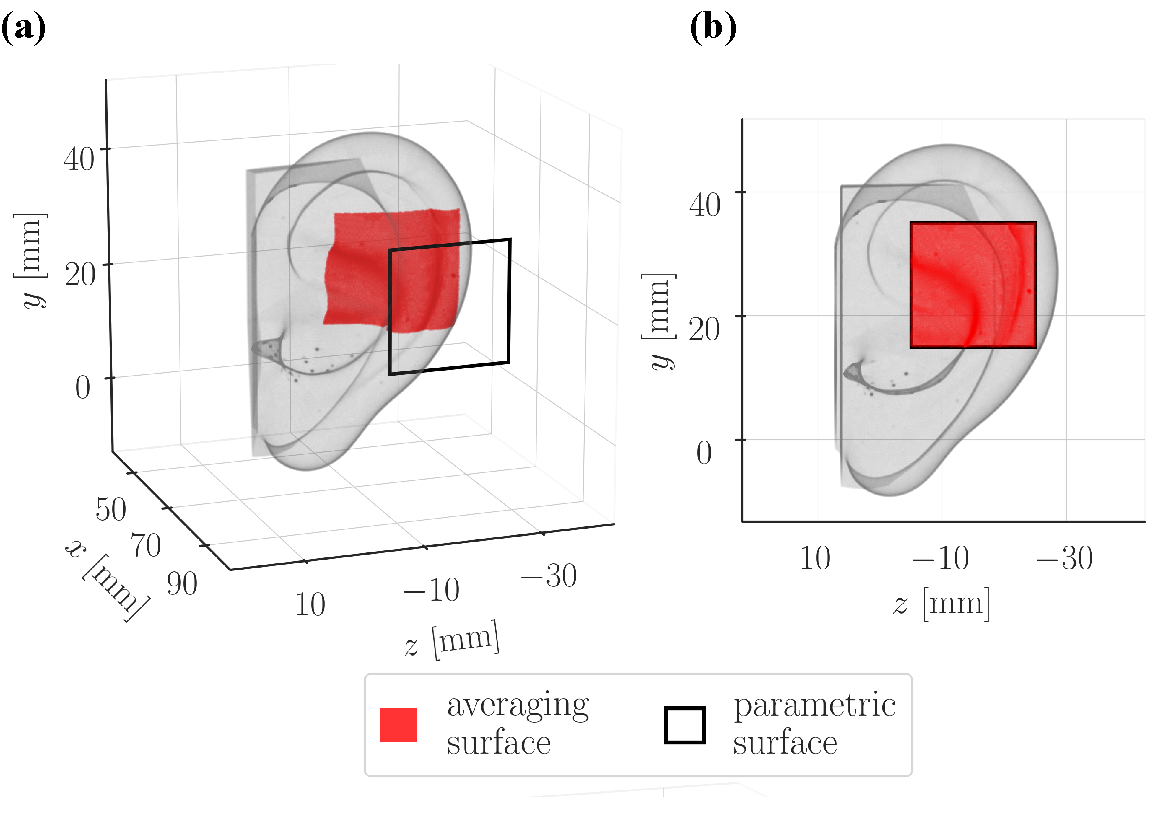
\includegraphics[width=0.8\textwidth]{artwork/Kapetanovic2022Assessment_figure2.pdf}
    \caption{Figure 2. in~\cite{Kapetanovic2022AssessmentJERM}: ``Conformal surface and its corresponding 2-D parametric projection of \SI{4}{\cm\squared} area. (a) 3-D view, and (b) The plane-wave incidence point of view.''}
    \label{fig:kapetanovic2022assessment}
\end{figure}
The results suggest that only a marginal difference between the values obtained from the two different definitions (within about \SI{6}{\percent}) is present regardless of the exposure scenarios.
However, by comparing the same results with common flat tissue-equivalent models, the spatial maximum \gls{apd} on the ear is up to about \SI{20}{\percent} larger regardless of definition.

In~\cite{Morimoto2022Assessment}, the effect of two distinct averaging shapes of the evaluation of the \gls{apd} and \gls{ipd} is investigated computationally.
The main goal of this study is to bridge the existing gap between exposure and product standards.
Namely, in two current international exposure limits, i.e., \gls{icnirp} guidelines~\cite{ICNIRP2020Guidelines} and the \gls{ieee} standard~\cite{IEEE2019Standard}, the averaging area for the assessment of the \gls{apd} and corresponding \gls{ipd} is square shaped and set to \SI{4}{\cm\squared} at the \SIrange[range-units=single,range-phrase=--]{6}{300}{\GHz} range.
Additionally, above \SI{30}{\GHz}, a square-shaped averaging area of \SI{1}{\cm\squared} should be considered as well to account for the small beam formation at the exposed surface.
On the other hand, international standards for product assessment~\cite{IEC2018,IEC2022part1,IEC2022part2} prescribe an averaging scheme of a circular shape in case of non-planar exposed surface for both computational and experimental evaluation of the \gls{ipd} to account the uncertainty during the assessment.
For this inconsistency, authors argue that it is of utmost importance to appropriately define the shape of the averaging surface following the exposure standard rather than product standard as the latter is based on the limits prescribed in exposure standards.
Furthermore, in the \gls{icnirp} guidelines on limits of exposure to laser radiation~\cite{ICNIRP2013Guidelines} that pertains to frequencies above \SI{300}{\GHz}, it is also a circular shape that is suggested as probe aperture for measurements of the power density at the surface of exposed tissue.
For this reason also, authors argue again that the discontinuation of the use of the averaging shape is of special interest.
In this study, planar homogeneous tissue-equivalent models and the human anatomical model are used to assess compliance and compute the the difference in the spatially averaged dosimetric quantities between square and circular averaging shapes by means of the heating factor.
Both models are irradiated by using dipole antennas and dipole arrays in various configuration at different distances.
The maximum differences in heating factors of the \gls{apd} and \gls{ipd} for square and circular averaging areas are marginal (in both cases about \SI{4}{\percent}) at the antenna-to-tissue separation distance $> \SI{5}{\mm}$ and are pronounced mostly when the surface of the model is elliptical in shape.
Overall, the heating factors for both the \gls{apd} and \gls{ipd} averaged on a circular averaging shape are conservative in comparison to those obtained for a square averaging shape up to \SI{300}{\GHz}.
The only exception is then the incident angle of the beam is within the \SIrange[range-units=single,range-phrase=--]{30}{60}{\degree} range.

This subject is further explored in a small scale study in~\cite{Kapetanovic2022Assessment} where the assessment of the spatially-averaged \gls{apd} on a realistic ear model is provided.
The \gls{em} analysis is performed computationally for plane wave exposure at \SI{60}{\GHz}.
The effect of the averaging area shape by using the same shape types, i.e., the square and disk both with the area of \SI{1}{\cm\squared}, as in~\cite{Morimoto2022Assessment} on the \gls{apd} is investigated.
By comparing the values of the \gls{apd} with different polarization of the impinging plane wave, a substantial relative difference of \SI{14}{\percent} between transverse electric and magnetic polarization is present on a circular averaging area.
On the other hand, negligible differences (up to \SI{2}{\percent}) exist between the \gls{apd} on different averaging area shape.
Authors conclude that, according to the studied exposure scenarios, variations in \gls{apd} as a function of the averaging surface shape are less significant than those related to the electric characteristics of the incident field.

% chapter 5 - conclusion
\clearpage
\chapter{Conclusion}

With ever increasing number of \gls{5g} personal wireless devices operating above \SI{6}{\GHz}, there is a growing public concern about biological safety.
Thus, the \gls{icnirp} guidelines and \gls{ieee} standard for limiting exposure to \gls{em} fields have recently undergone major revisions.
One prominent technical update is the introduction of the newly defined physical quantity as the \gls{br}/\gls{drl}.
Namely, the \gls{apd} is now to be used for compliance assessment above \SI{6}{\GHz}.
Because its use is limited for local exposure, the \gls{apd} should be spatially averaged over \SI{4}{\cm\squared} control surface that lies on the front face of the tissue equivalent block.

The \gls{apd} and its free space counterpart \gls{ipd}, that is to be used for exposure assessment as the \gls{rl}/\gls{erl}, are proven to be valid proxies for maximum temperature rise on the exposed skin surface.
However, if the curvature of the tissue is pronounced, recent literature points to the fact that the extracted values can be underestimated by using planar averaging surfaces.
Still, most research in computational dosimetry on which the international exposure limits are based use flat tissue-equivalent models to simplify the problem geometry.
Depending on the ratio of the penetration depth and local curvature radius of the exposed tissue, this approach may lead to inaccurate estimates of the power absorption.
It is thus of utmost importance to account for the geometrical complexity of the exposed models.

This work is the result of an effort to review the complete literature that deals closely with the evaluation of area-averaged dosimetric quantities.
Of special interest are the averaging technique itself through the lens of numerical approximation of the relevant surface integrals.
The generation of the parametric surface on which the integration points are distributed, the shape and dimensions of that surface, the influence of curvature and other realistic morphological features during parametrization from 3-D to 2-D space, etc., are all topics that are also taken into account.
Before that, the general introduction to human exposure to \gls{em} fields, especially in the era of \gls{5g}, is given.
Loosely defined concepts of the derivation of the \gls{apd} from \gls{sar} used as the \gls{br}/\gls{drl} at lower frequencies, as well as the equivalence of different prescribed definitions of both the \gls{apd} and \gls{ipd} are elaborated in detail and supported by relevant literature.
Advanced numerical approaches for the assessment of the \gls{apd} and \gls{ipd} on conformal surfaces of anatomical human models are addressed.

This work is in accordance with discussions currently held within the Working Group 7 of the \gls{ieee} international committee on \gls{em} safety (Technical Committee 95, Subcommittee 6).
The goal of this working group is to resolve uncertainties related to numerical models and integration methods, but also to the geometrical shape of the averaging surface for the assessment of the \gls{apd} and \gls{ipd} at the \SIrange[range-units=single,range-phrase=--]{6}{300}{\GHz} range.
Special emphasis is on the average schemes and assessment methods of the \gls{apd} on non-planar body parts.
Motivated by previous topics, this work finally starts the discussion of numerical approximation of surface integrals across non-canonical surfaces of morphologically-accurate tissue models.
This is left as an open problem to be addressed through future work.


% references - add to ToC without the number of chapter
\clearpage
\phantomsection
\addcontentsline{toc}{chapter}{Bibliography}
\markboth{Bibliography}{Bibliography}
\printbibliography

% abbreviations - add to ToC without the number of chapter
\phantomsection
\addcontentsline{toc}{chapter}{Acronyms}
\markboth{Acronyms}{Acronyms}
\printglossaries

% abstract - add to ToC without the number of chapter
\clearpage
\phantomsection
\addcontentsline{toc}{chapter}{Abstract}
\markboth{Abstract}{Abstract}
\chapter*{Abstract}

With the increased use of \gls{5g} personal wireless devices in close proximity to the human body, international exposure limits have been recently updated to take into account exposure above \SI{6}{\GHz}, including the entirety of the \gls{mmw} spectrum.
The limits for local steady-state exposure are given in terms of the \gls{apd} and its free space counterpart -- the \gls{ipd}.
Both quantities require spatial averaging on the control evaluation plane whose surface area depends on the frequency of the incident \gls{em} field.
Spatially-averaged power densities have been proven to be valid proxies for local temperature rise on exposed surfaces with no pronounced curvature.
However, when local curvature radii on the surface are of the same order of magnitude as the wavelength of the incident wave, accuracy of the extracted dosimetric quantities is compromised.
This is most often manifested through the underestimation of actual values, which leads to the inability to demonstrate compliance.
This work presents a literature review that pertains to the current approach in the spatial averaging of power densities for local exposure above \SI{6}{\GHz}.
In addition, proposed potential upgrades in terms of spatial averaging on non-planar surfaces are addressed with a special emphasis on canonical geometries such as the sphere and cylinder.

% abstract in Croatian - add to ToC without the number of chapter
\clearpage
\phantomsection
\addcontentsline{toc}{chapter}{Sažetak}
\markboth{Sažetak}{Sažetak}
\input{chapters/06_Sažetak}

\end{document}